% =====================================================================
%  Chapter 18: The Generalized Stokes Theorem
%  Sections 18.1 and 18.2
% =====================================================================

\chapter{The Generalized Stokes Theorem}
\label{ch:18}

Chapter \ref{ch:17} focused on the derivative side of the story.  We learned that one
symbol,
\[
    d,
\]
contains gradient, curl, and divergence, depending on the degree of the form:
\[
    f\mapsto df,\qquad
    \omega\mapsto d\omega,\qquad
    \Phi\mapsto d\Phi.
\]

The other side of the story is the boundary.

A boundary is not only a shape.  It carries signs and directions.  The right endpoint of
an interval is positive and the left endpoint is negative.  The boundary of a plane region
is walked in a chosen direction.  A surface has a chosen side.  A solid has an outward
surface.

The generalized Stokes theorem is short:
\[
    \int_{\partial M}\omega=\int_M d\omega.
\]
But that sentence only makes sense after we know what \(\partial M\) means and how it
is oriented.

\section{Boundaries and orientation}
\label{sec:18.1}

A form changes sign when orientation reverses.  So before we state the theorem, we
must make the signs automatic.  The boundary of an interval, a region, a surface, or a
solid should inherit its orientation from the object it bounds.

\subsection{Oriented intervals and endpoints}

Start with the old one-dimensional picture.

The interval
\[
    I=[a,b]
\]
is oriented from left to right.  Its boundary consists of two endpoints, but the endpoints
do not have the same sign:
\[
\boxed{
    \partial[a,b]=\{b\}-\{a\}.
}
\]
The right endpoint is positive.  The left endpoint is negative.

This is exactly the sign pattern in the Fundamental Theorem of Calculus:
\[
    \int_a^b f'(x)\,dx=f(b)-f(a).
\]
In forms language, \(f\) is a \(0\)-form and
\[
    \int_{\partial[a,b]} f=f(b)-f(a).
\]

\begin{example}[The boundary of an interval]
Let
\[
    I=[2,5]
\]
with the usual left-to-right orientation, and let
\[
    f(x)=x^2+1.
\]
Then
\[
    \partial I=\{5\}-\{2\}.
\]
So
\[
\begin{aligned}
    \int_{\partial I} f
    &=
    f(5)-f(2)\\
    &=
    26-5\\
    &=
    21.
\end{aligned}
\]

If the same interval is given the opposite orientation, then its boundary becomes
\[
    \{2\}-\{5\},
\]
and the integral becomes
\[
    -21.
\]
\end{example}

A point by itself has no direction to walk.  Its orientation is only a sign:
\[
    +P
    \qquad\text{or}\qquad
    -P.
\]
That is enough for \(0\)-forms.

\begin{definition}[Oriented boundary of an interval]
If the interval \([a,b]\) is oriented from \(a\) to \(b\), then
\[
\boxed{
    \partial[a,b]=\{b\}-\{a\}.
}
\]
Reversing the orientation reverses the signs of the endpoints.
\end{definition}

The sign convention can be remembered by the word ``outward.''  At the right endpoint,
the outward direction points in the positive direction of the interval.  At the left
endpoint, the outward direction points in the negative direction.  So the right endpoint
gets \(+\), and the left endpoint gets \(-\).

\subsection{Oriented plane regions and boundary curves}

A region in the \(xy\)-plane has the standard orientation
\[
    dx\wedge dy.
\]
This means that the ordered pair of directions
\[
    \text{positive }x\text{-direction first, positive }y\text{-direction second}
\]
is positive.

The boundary of such a region is oriented so that the region stays on your left as you
walk along the boundary.

For a region without holes, this means counterclockwise.

\begin{figure}[h]
\centering
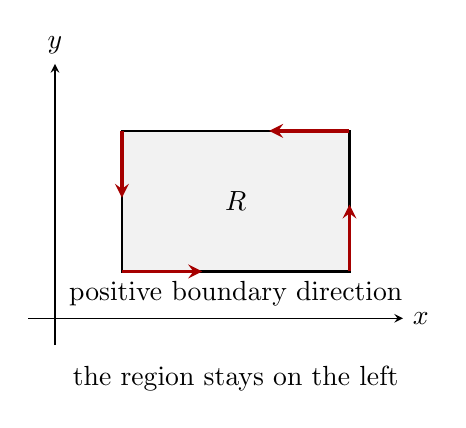
\begin{tikzpicture}[scale=0.85, >=stealth]
    \draw[->] (-0.4,0) -- (5.2,0) node[right] {\(x\)};
    \draw[->] (0,-0.4) -- (0,3.8) node[above] {\(y\)};

    \draw[fill=gray!10, thick] (1,0.7) rectangle (4.4,2.8);

    \draw[->, very thick, red!65!black] (1,0.7) -- (2.2,0.7);
    \draw[->, very thick, red!65!black] (4.4,0.7) -- (4.4,1.7);
    \draw[->, very thick, red!65!black] (4.4,2.8) -- (3.2,2.8);
    \draw[->, very thick, red!65!black] (1,2.8) -- (1,1.8);

    \node at (2.7,1.75) {\(R\)};
    \node[below] at (2.7,0.7) {positive boundary direction};

    \node at (2.7,-0.9) {the region stays on the left};
\end{tikzpicture}
\caption{A positively oriented plane boundary keeps the region on the left.}
\end{figure}

\begin{example}[A rectangle and its positive boundary]
Let
\[
    R=[0,4]\times[0,3],
\]
oriented by
\[
    dx\wedge dy.
\]
Then \(\partial R\) is the rectangle walked counterclockwise:
\[
    (0,0)\to(4,0)\to(4,3)\to(0,3)\to(0,0).
\]

If
\[
    \omega=x\,dy,
\]
then the bottom and top edges contribute \(0\), because \(dy=0\) there.  The right edge
has
\[
    x=4,\qquad 0\le y\le3,
\]
so
\[
    \int_{\text{right edge}}x\,dy=\int_0^3 4\,dy=12.
\]
The left edge has
\[
    x=0,
\]
so it contributes \(0\).  Therefore
\[
\boxed{
    \int_{\partial R} x\,dy=12.
}
\]
If we walk the rectangle clockwise, the answer becomes
\[
    -12.
\]
\end{example}

For a region with a hole, the same ``region on the left'' rule gives two different-looking
directions.

The outer boundary is counterclockwise.  The inner boundary is clockwise.

\begin{figure}[h]
\centering
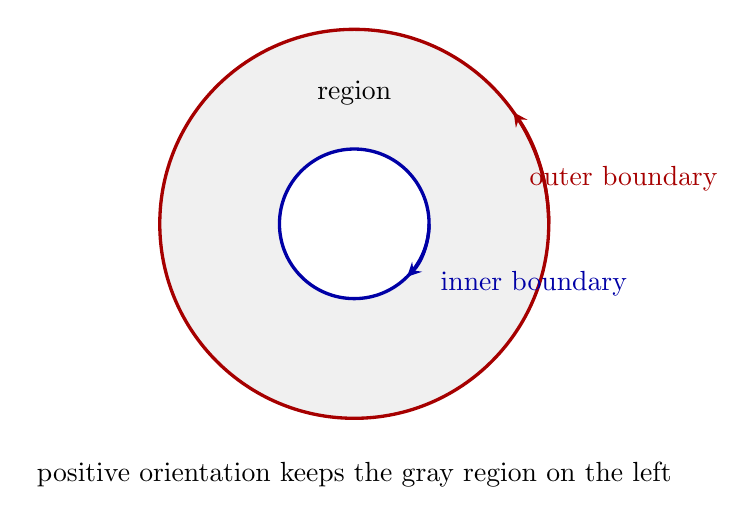
\begin{tikzpicture}[scale=0.95, >=stealth]
    \draw[fill=gray!12, even odd rule]
        (0,0) circle (2.6)
        (0,0) circle (1.0);

    \draw[very thick, red!65!black] (0,0) circle (2.6);
    \draw[->, very thick, red!65!black]
        (2.6,0) arc[start angle=0,end angle=35,radius=2.6];

    \draw[very thick, blue!65!black] (0,0) circle (1.0);
    \draw[->, very thick, blue!65!black]
        (1,0) arc[start angle=0,end angle=-45,radius=1.0];

    \node at (0,1.75) {region};
    \node[red!65!black] at (3.6,0.6) {outer boundary};
    \node[blue!65!black] at (2.4,-0.8) {inner boundary};

    \node at (0,-3.35) {positive orientation keeps the gray region on the left};
\end{tikzpicture}
\caption{The inner boundary of a positively oriented annulus is walked clockwise.}
\end{figure}

This is not a special exception.  It is the same rule.  If you walk around the hole
clockwise, the material of the annulus stays on your left.

\begin{definition}[Positive boundary orientation in the plane]
Let \(R\) be a plane region oriented by \(dx\wedge dy\).  The positive orientation of
\(\partial R\) is the one for which the region stays on the left as the boundary is
traveled.

For a region without holes, this is counterclockwise.  For an inner boundary around a
hole, this is clockwise.
\end{definition}

\subsection{Oriented surfaces and boundary curves}

A surface in space is oriented by choosing one of its two sides.  Equivalently, we choose
a continuous unit normal vector field
\[
    \mathbf n
\]
on the surface.

For a parametrized surface
\[
    \mathbf r(u,v),
\]
the normal direction attached to the parameter order \((u,v)\) is
\[
    \mathbf r_u\times \mathbf r_v.
\]
Swapping the parameters reverses the orientation:
\[
    \mathbf r_v\times \mathbf r_u
    =
    -\mathbf r_u\times \mathbf r_v.
\]

Once the surface orientation is chosen, the boundary curve orientation is forced.

\begin{example}[A disk with two possible orientations]
Let \(D\) be the unit disk in the \(xy\)-plane:
\[
    x^2+y^2\le1.
\]

If \(D\) is oriented by the upward normal
\[
    \mathbf n=\mathbf k,
\]
then its boundary circle is oriented counterclockwise when viewed from above:
\[
    \mathbf r(t)=(\cos t,\sin t,0),
    \qquad
    0\le t\le2\pi.
\]

If \(D\) is oriented by the downward normal
\[
    \mathbf n=-\mathbf k,
\]
then the same boundary circle is oriented clockwise when viewed from above:
\[
    \mathbf r(t)=(\cos t,-\sin t,0),
    \qquad
    0\le t\le2\pi.
\]
\end{example}

The rule is the right-hand rule.

Point your right thumb in the chosen normal direction.  Your fingers curl in the positive
boundary direction.

\begin{figure}[h]
\centering
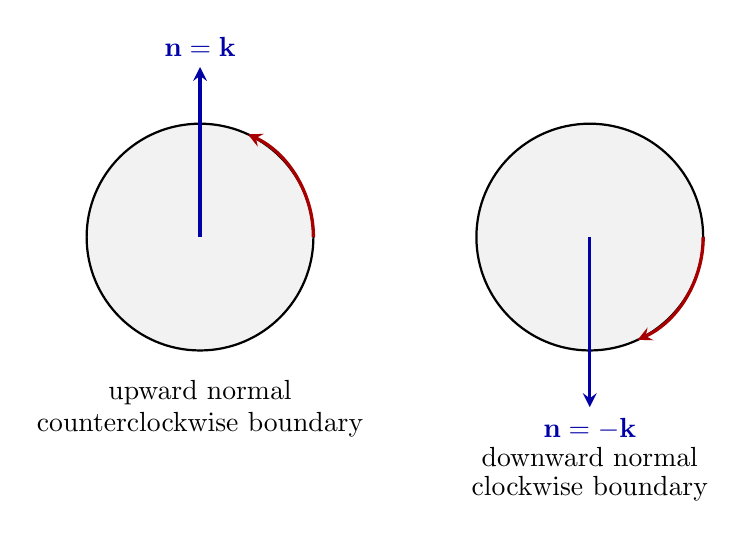
\begin{tikzpicture}[scale=0.9, >=stealth]
    \begin{scope}
        \draw[fill=gray!10, thick] (0,0) circle (1.6);
        \draw[->, very thick, red!65!black]
            (1.6,0) arc[start angle=0,end angle=65,radius=1.6];

        \draw[->, very thick, blue!65!black] (0,0) -- (0,2.4)
            node[above] {\(\mathbf n=\mathbf k\)};

        \node at (0,-2.2) {upward normal};
        \node at (0,-2.65) {counterclockwise boundary};
    \end{scope}

    \begin{scope}[shift={(5.5,0)}]
        \draw[fill=gray!10, thick] (0,0) circle (1.6);
        \draw[->, very thick, red!65!black]
            (1.6,0) arc[start angle=0,end angle=-65,radius=1.6];

        \draw[->, very thick, blue!65!black] (0,0) -- (0,-2.4)
            node[below] {\(\mathbf n=-\mathbf k\)};

        \node at (0,-3.1) {downward normal};
        \node  at (0,-3.55) {clockwise boundary};
    \end{scope}
\end{tikzpicture}
\caption{Changing the surface normal reverses the boundary orientation.}
\end{figure}

There is also a version of the ``region on the left'' rule for surfaces.

Imagine standing on the surface with your head pointing in the chosen normal direction.
Walk along the boundary in the positive direction.  The surface should stay on your
left.

\begin{definition}[Boundary orientation of an oriented surface]
Let \(S\) be an oriented surface with chosen normal direction \(\mathbf n\).  The positive
orientation of \(\partial S\) is the direction given by the right-hand rule: the thumb
points in the direction of \(\mathbf n\), and the fingers curl in the positive boundary
direction.

Equivalently, when walking along the boundary with head in the normal direction, the
surface stays on the left.
\end{definition}

This is the orientation used in Stokes' theorem:
\[
    \int_{\partial S}\omega=\int_S d\omega.
\]
The sign of the boundary integral depends on the side of the surface we chose.

\subsection{Oriented solids and boundary surfaces}

A solid region in ordinary space has the standard orientation
\[
    dx\wedge dy\wedge dz.
\]
The boundary of a solid is a surface, and its positive orientation is the outward one.

This is the orientation used for flux.  A flux integral over the boundary of a solid uses
the outward normal.

\begin{example}[The boundary orientation of a box]
Let
\[
    E=[0,2]\times[0,3]\times[0,4].
\]
The boundary \(\partial E\) has six faces.  Each face is oriented by its outward normal.

\[
\begin{array}{c|c|c}
\text{Face} & \text{Outward normal} & \text{Positive area form on the face} \\ \hline
x=2 & \mathbf i & dy\wedge dz\\[1mm]
x=0 & -\mathbf i & dz\wedge dy\\[1mm]
y=3 & \mathbf j & dz\wedge dx\\[1mm]
y=0 & -\mathbf j & dx\wedge dz\\[1mm]
z=4 & \mathbf k & dx\wedge dy\\[1mm]
z=0 & -\mathbf k & dy\wedge dx
\end{array}
\]

For instance, the top face \(z=4\) has outward normal \(\mathbf k\), so its positive
surface orientation is \(dx\wedge dy\).  The bottom face \(z=0\) has outward normal
\(-\mathbf k\), so its positive surface orientation is \(dy\wedge dx=-dx\wedge dy\).
\end{example}

This sign pattern is not arbitrary.  It comes from the same ``outward first'' rule that
worked for intervals and plane regions.

\subsection{The outward-first convention}

All boundary orientations in this book come from one convention.

\begin{definition}[Outward-first convention]
Let \(M\) be an oriented \(k\)-dimensional object, where \(k=1,2,\) or \(3\).  At a
smooth boundary point, let
\[
    \nu_{\text{out}}
\]
be the outward direction normal to the boundary but tangent to \(M\).

A list of boundary tangent vectors
\[
    \mathbf v_1,\ldots,\mathbf v_{k-1}
\]
is positively oriented on \(\partial M\) if the list
\[
\boxed{
    \nu_{\text{out}},\mathbf v_1,\ldots,\mathbf v_{k-1}
}
\]
is positively oriented in \(M\).
\end{definition}

This convention may look abstract, so let us test it in the three familiar cases.

\[
\begin{array}{c|c|c}
M & \nu_{\text{out}} & \text{Resulting boundary orientation} \\ \hline
[a,b] &
\begin{array}{c}
- \text{ direction at }a\\
+ \text{ direction at }b
\end{array}
&
\partial[a,b]=\{b\}-\{a\}
\\[5mm]
\text{plane region with }dx\wedge dy &
\text{outward direction in the plane} &
\text{region stays on the left}
\\[2mm]
\text{surface with normal }\mathbf n &
\text{outward direction along the surface} &
\text{right-hand rule around the boundary}
\\[2mm]
\text{solid with }dx\wedge dy\wedge dz &
\text{outward normal in space} &
\text{outward-oriented boundary surface}
\end{array}
\]

The theorem needs exactly these signs.  If one sign is reversed, the two sides of
Stokes' theorem disagree by a minus sign.

The boundary has now become a signed object.  That is the missing piece.  A form lives
on the boundary, its derivative lives inside, and the orientations are ready to make the
two integrals comparable.

The next step is to state the theorem that has been hiding behind the Fundamental
Theorem of Calculus, Green's theorem, Stokes' theorem, and the divergence theorem.

\section{The theorem}
\label{sec:18.2}

Section \ref{sec:18.1} fixed the signs on boundaries.  Chapter \ref{ch:17} fixed the
meaning of \(d\).  The generalized Stokes theorem simply puts those two pieces in one
sentence.

Before stating it, let us watch it work in one familiar rectangle.

\subsection{A rectangle that already knows the theorem}

Let
\[
    R=[0,4]\times[0,3]
\]
with its standard orientation
\[
    dx\wedge dy.
\]
Its boundary is oriented counterclockwise.

Take the \(1\)-form
\[
    \omega=x\,dy.
\]
We computed in Section \ref{sec:18.1} that
\[
    \int_{\partial R} x\,dy=12.
\]

Now compute the exterior derivative:
\[
    d\omega=d(x\,dy).
\]
Since
\[
    dx\wedge dy
\]
is the area form,
\[
    d(x\,dy)=dx\wedge dy.
\]
Therefore
\[
\begin{aligned}
    \int_R d\omega
    &=
    \int_R dx\wedge dy\\
    &=
    \operatorname{Area}(R)\\
    &=
    12.
\end{aligned}
\]

So
\[
\boxed{
    \int_{\partial R}\omega=\int_R d\omega.
}
\]

The boundary integral added \(x\,dy\) around the edge.  The interior integral added
\(dx\wedge dy\) across the rectangle.  They gave the same number.

Nothing in this calculation depended on a hidden trick.  The right edge of the rectangle
carried all the boundary contribution, and the interior area had the same total size.
For a more complicated \(1\)-form, the same comparison happens locally on tiny
rectangles.  The exterior derivative measures the boundary circulation per unit area.

\subsection{The statement}

Here is the theorem in the form we will use.

\begin{theorem}[Generalized Stokes theorem, dimensions \(1\), \(2\), and \(3\)]
Let \(M\) be an oriented, compact, piecewise smooth \(k\)-dimensional object, with
\(k=1,2,\) or \(3\).  Give \(\partial M\) the induced boundary orientation from
Section \ref{sec:18.1}.

Let \(\omega\) be a \(C^1\) differential form of degree \(k-1\), defined on an open set
containing \(M\).  Then
\[
\boxed{
    \int_{\partial M}\omega=\int_M d\omega.
}
\]

If
\[
    \partial M=\emptyset,
\]
then the left side is defined to be \(0\).
\end{theorem}

The theorem is short, but every word is doing work.

\[
\begin{array}{c|c}
\text{Phrase} & \text{Meaning in this book} \\ \hline
\text{oriented} & \text{directions or sides have been chosen}\\[1mm]
\text{compact} & \text{finite, closed, bounded pieces in our examples}\\[1mm]
\text{piecewise smooth} & \text{smooth pieces are allowed to meet at corners}\\[1mm]
\omega\text{ has degree }k-1 & \omega\text{ can be integrated over }\partial M\\[1mm]
d\omega\text{ has degree }k & d\omega\text{ can be integrated over }M\\[1mm]
\omega\text{ is defined near }M & \text{there are no hidden singularities inside}
\end{array}
\]

\subsection{What kind of object \(M\) is}

The letter \(M\) is a common name for the object being integrated over.  It does not
force us into a new abstract world.  In this book, \(M\) will be one of the following
kinds of pieces.

\[
\begin{array}{c|c|c}
k & M & \partial M \\ \hline
1 &
\text{oriented interval or curve segment} &
\text{signed endpoints}
\\[1mm]
2 &
\text{oriented plane region} &
\text{oriented boundary curves}
\\[1mm]
2 &
\text{oriented surface in space} &
\text{oriented boundary curves}
\\[1mm]
3 &
\text{oriented solid region in space} &
\text{oriented boundary surfaces}
\end{array}
\]

A rectangle, a disk, an annulus, a cylinder side, a hemisphere, a box, and a solid ball
all fit this language.

Corners are allowed.  A rectangle is not smooth at its four corners, but it is made of
smooth sides.  A box is not smooth along its edges, but it is made of smooth faces.
That is what ``piecewise smooth'' means here.

A sphere considered as a surface has no boundary curve:
\[
    \partial S=\emptyset.
\]
A solid ball has boundary:
\[
    \partial E=\text{the sphere}.
\]
The same sphere can appear in two different roles, and the theorem reads it differently
depending on the dimension of \(M\).

\subsection{What kind of object \(\omega\) is}

The form \(\omega\) always has one degree less than \(M\).

If \(M\) is one-dimensional, then \(\omega\) is a \(0\)-form, which means a function.
If \(M\) is two-dimensional, then \(\omega\) is a \(1\)-form.  If \(M\) is
three-dimensional, then \(\omega\) is a \(2\)-form.

\[
\begin{array}{c|c|c|l}
\dim M & \omega & d\omega & \text{Classical name} \\ \hline
1 &
f &
df &
\begin{tabular}{@{}l@{}}Fundamental Theorem \\ of Calculus\end{tabular}
\\[4mm]
2 &
P\,dx+Q\,dy &
(Q_x-P_y)\,dx\wedge dy &
\begin{tabular}{@{}l@{}}Green's theorem \\ in the plane\end{tabular}
\\[4mm]
2 &
P\,dx+Q\,dy+R\,dz &
d\omega &
\begin{tabular}{@{}l@{}}Stokes' theorem \\ on a surface\end{tabular}
\\[4mm]
3 &
\begin{aligned}
    P\,dy\wedge dz &+ Q\,dz\wedge dx \\
    &+ R\,dx\wedge dy
\end{aligned} &
\begin{aligned}
    &(P_x+Q_y+R_z) \\
    &\,dx\wedge dy\wedge dz
\end{aligned} &
\text{Divergence theorem}
\end{array}
\]

This table is the whole chapter in compressed form.  The next sections will unpack
each row.

\subsection{Why the dimensions match}

The theorem says
\[
    \int_{\partial M}\omega=\int_M d\omega.
\]
The two integrals live in different places, but their dimensions match perfectly.

If
\[
    \dim M=k,
\]
then
\[
    \dim(\partial M)=k-1.
\]
The form \(\omega\) has degree \(k-1\), so it can be integrated over \(\partial M\).
The exterior derivative \(d\omega\) has degree \(k\), so it can be integrated over \(M\).

\[
\boxed{
\begin{array}{ccc}
\omega & \text{lives on} & \partial M\\[1mm]
d\omega & \text{lives on} & M
\end{array}
}
\]

That is the reason \(d\) raises degree by one.  The derivative inside the region must be
one dimension higher than the form on the boundary.

\subsection{Why the hypotheses are needed}

The theorem is powerful because it is precise.  If we drop its conditions carelessly, the
formula can lose meaning or give the wrong sign.

\subsubsection*{The boundary orientation must be induced}

Take the unit square
\[
    R=[0,1]\times[0,1]
\]
with the usual orientation \(dx\wedge dy\), and take
\[
    \omega=x\,dy.
\]
Then
\[
    d\omega=dx\wedge dy,
\]
so
\[
    \int_R d\omega=1.
\]

With the induced boundary orientation, \(\partial R\) is counterclockwise and
\[
    \int_{\partial R}\omega=1.
\]
But if we walk the boundary clockwise, then
\[
    \int_{-\partial R}\omega=-1.
\]
So the formula would say
\[
    -1=1,
\]
which is false.

The theorem did not fail.  We used the wrong boundary orientation.

\subsubsection*{Every boundary component must be included}

Let
\[
    A=\{(x,y):1\le x^2+y^2\le4\}
\]
be the annulus between the circles of radius \(1\) and \(2\).  Use the standard
orientation \(dx\wedge dy\), and again take
\[
    \omega=x\,dy.
\]
Then
\[
    d\omega=dx\wedge dy,
\]
so
\[
    \int_A d\omega=\operatorname{Area}(A)=4\pi-\pi=3\pi.
\]

Now compute the boundary integral.  The outer circle is counterclockwise, and the inner
circle is clockwise.

On a counterclockwise circle of radius \(r\),
\[
    x=r\cos t,\qquad y=r\sin t,
\]
so
\[
    dy=r\cos t\,dt.
\]
Thus
\[
\begin{aligned}
    \int x\,dy
    &=
    \int_0^{2\pi} r^2\cos^2 t\,dt\\
    &=
    \pi r^2.
\end{aligned}
\]
The outer circle contributes
\[
    4\pi.
\]
The inner circle is oriented clockwise, so it contributes
\[
    -\pi.
\]
Therefore
\[
    \int_{\partial A}\omega=4\pi-\pi=3\pi.
\]

If we forgot the inner boundary, we would get
\[
    4\pi,
\]
which is wrong.  Holes have boundary curves too, and their orientations matter.

\subsubsection*{The form must be defined on the whole region}

Consider the \(1\)-form on the punctured plane
\[
    \eta=
    \frac{-y}{x^2+y^2}\,dx
    +
    \frac{x}{x^2+y^2}\,dy.
\]
Chapter \ref{ch:17} showed that this form is closed where it is defined:
\[
    d\eta=0
    \qquad
    \text{on }
    \mathbb R^2\setminus\{(0,0)\}.
\]

On the unit circle
\[
    x=\cos t,\qquad y=\sin t,
\]
we have
\[
    dx=-\sin t\,dt,\qquad dy=\cos t\,dt.
\]
So
\[
\begin{aligned}
    \eta
    &=
    (-\sin t)(-\sin t\,dt)+(\cos t)(\cos t\,dt)\\
    &=
    dt.
\end{aligned}
\]
Therefore
\[
    \int_{x^2+y^2=1}\eta=\int_0^{2\pi}dt=2\pi.
\]

A careless use of Stokes' theorem on the unit disk would say
\[
    \int_{\partial D}\eta=\int_D d\eta=0.
\]
But this is not allowed.  The form \(\eta\) is not defined at the origin, and the origin
lies inside the disk.

The missing point is not harmless.  The boundary circle detects it.

\subsubsection*{The smoothness assumptions keep the integrals meaningful}

The theorem asks for \(\omega\) to be \(C^1\).  This guarantees that \(d\omega\) exists
and is continuous.

For example,
\[
    \omega=|x|\,dy
\]
is not \(C^1\) on any region crossing the line \(x=0\).  The derivative of \(|x|\) is not
defined at \(x=0\), so the expression
\[
    d\omega
\]
is not defined by the rules of this book on that line.

Some rough cases can be handled by more advanced versions of Stokes' theorem.  But
the theorem stated here is a theorem for the objects we know how to integrate.

The same warning applies to the boundary.  A polygon is fine, because it is made from
smooth pieces.  A cube is fine, because it is made from smooth faces.  A wildly jagged
fractal boundary has no tangent direction at most points, so our line integral along it
has not been defined.

\subsection{Why the theorem is believable}

The proof idea is already visible in a grid.

Cut a plane region into many small rectangles.  On each small rectangle,
\[
    \int_{\partial(\text{small rectangle})}\omega
\]
measures the local boundary circulation.  The exterior derivative \(d\omega\) measures
the same local circulation per unit area, so
\[
    \int_{\partial(\text{small rectangle})}\omega
    =
    \int_{\text{small rectangle}}d\omega
\]
for the ideal small piece.

Now add all small rectangles.

Every interior edge is walked twice, once in each direction.  A \(1\)-form changes sign
when direction reverses, so the two contributions cancel.  Only the outside boundary
remains.

\begin{figure}[h]
\centering
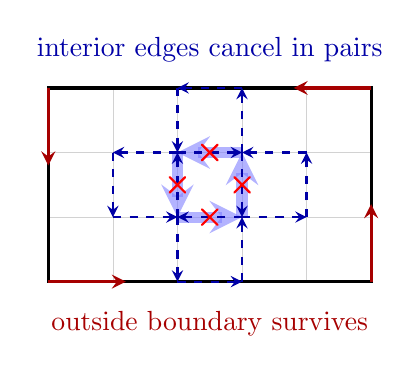
\begin{tikzpicture}[scale=0.82, >=stealth]
    \draw[step=1, gray!35, very thin] (0,0) grid (5,3);

    \draw[very thick] (0,0) rectangle (5,3);

    % Outer boundary arrows
    \draw[->, very thick, red!65!black] (0,0) -- (1.2,0);
    \draw[->, very thick, red!65!black] (5,0) -- (5,1.2);
    \draw[->, very thick, red!65!black] (5,3) -- (3.8,3);
    \draw[->, very thick, red!65!black] (0,3) -- (0,1.8);

    % Central square (thick, semi-transparent)
    % Oriented counterclockwise
    \draw[->, line width=4pt, blue!50, opacity=0.6] (2,1) -- (3,1);
    \draw[->, line width=4pt, blue!50, opacity=0.6] (3,1) -- (3,2);
    \draw[->, line width=4pt, blue!50, opacity=0.6] (3,2) -- (2,2);
    \draw[->, line width=4pt, blue!50, opacity=0.6] (2,2) -- (2,1);

    % Four adjacent squares (dashed arrows, oriented counterclockwise)
    
    % Bottom neighbor
    \draw[->, thick, dashed, blue!65!black] (2,0) -- (3,0);
    \draw[->, thick, dashed, blue!65!black] (3,0) -- (3,1);
    \draw[->, thick, dashed, blue!65!black] (3,1) -- (2,1); % Cancels central bottom edge
    \draw[->, thick, dashed, blue!65!black] (2,1) -- (2,0);

    % Right neighbor
    \draw[->, thick, dashed, blue!65!black] (3,1) -- (4,1);
    \draw[->, thick, dashed, blue!65!black] (4,1) -- (4,2);
    \draw[->, thick, dashed, blue!65!black] (4,2) -- (3,2);
    \draw[->, thick, dashed, blue!65!black] (3,2) -- (3,1); % Cancels central right edge

    % Top neighbor
    \draw[->, thick, dashed, blue!65!black] (2,2) -- (3,2); % Cancels central top edge
    \draw[->, thick, dashed, blue!65!black] (3,2) -- (3,3);
    \draw[->, thick, dashed, blue!65!black] (3,3) -- (2,3);
    \draw[->, thick, dashed, blue!65!black] (2,3) -- (2,2);

    % Left neighbor
    \draw[->, thick, dashed, blue!65!black] (1,1) -- (2,1);
    \draw[->, thick, dashed, blue!65!black] (2,1) -- (2,2); % Cancels central left edge
    \draw[->, thick, dashed, blue!65!black] (2,2) -- (1,2);
    \draw[->, thick, dashed, blue!65!black] (1,2) -- (1,1);

    % Red crosses to visually mark the cancellations on the 4 shared edges
    \foreach \x/\y in {2.5/1, 3/1.5, 2.5/2, 2/1.5} {
        \draw[red, thick, line cap=round] (\x-0.12, \y-0.12) -- (\x+0.12, \y+0.12);
        \draw[red, thick, line cap=round] (\x-0.12, \y+0.12) -- (\x+0.12, \y-0.12);
    }

    \node[red!65!black] at (2.5,-0.65) {outside boundary survives};
    \node[blue!65!black] at (2.5,3.6) {interior edges cancel in pairs};
\end{tikzpicture}
\caption{When small pieces are added, interior boundary contributions cancel.}
\end{figure}

The same cancellation happens for intervals, surfaces, and solids.

For intervals, the interior endpoints cancel:
\[
    (f(x_1)-f(x_0))+(f(x_2)-f(x_1))+\cdots+(f(x_n)-f(x_{n-1}))
    =
    f(x_n)-f(x_0).
\]

For surfaces, interior curves cancel.  For solids, interior faces cancel.  Boundary is
what remains after all interior cancellations.

That is the heart of the generalized Stokes theorem.

The next sections will open the theorem one disguise at a time.  The first disguise is
the oldest one: a function on an interval, whose derivative adds up to
\[
    f(b)-f(a).
\]
The Fundamental Theorem of Calculus was already Stokes' theorem.  We just did not yet
have the language to say so.
\section{The Fundamental Theorem of Calculus as Stokes}
\label{sec:18.3}

The generalized Stokes theorem says
\[
    \int_{\partial M}\omega=\int_M d\omega.
\]
The shortest nontrivial case happens when \(M\) is an interval.  Then the boundary is
only two signed endpoints, and \(\omega\) is only a function.

That case is not a new theorem.  It is the Fundamental Theorem of Calculus.

\subsection{A changing temperature along a rod}

Imagine a thin metal rod lying along the \(x\)-axis from
\[
    x=1
    \qquad\text{to}\qquad
    x=4.
\]
The temperature along the rod is
\[
    T(x)=x^2+2x.
\]
Then
\[
    dT=T'(x)\,dx=(2x+2)\,dx.
\]

The interval
\[
    I=[1,4]
\]
is oriented from left to right.  Its boundary is
\[
    \partial I=\{4\}-\{1\}.
\]
So the boundary integral of the \(0\)-form \(T\) is
\[
\begin{aligned}
    \int_{\partial I}T
    &=
    T(4)-T(1)\\
    &=
    (16+8)-(1+2)\\
    &=
    21.
\end{aligned}
\]

Now integrate the derivative through the inside:
\[
\begin{aligned}
    \int_I dT
    &=
    \int_1^4 (2x+2)\,dx\\
    &=
    \left[x^2+2x\right]_1^4\\
    &=
    21.
\end{aligned}
\]
Thus
\[
\boxed{
    \int_{\partial I}T=\int_I dT.
}
\]

This is exactly Stokes' theorem:
\[
    \int_{\partial M}\omega=\int_M d\omega,
\]
with
\[
    M=I,
    \qquad
    \omega=T.
\]

\subsection{A \(0\)-form on an interval}

A \(0\)-form is a function.  On an interval,
\[
    \omega=f(x)
\]
is a \(0\)-form, and its exterior derivative is the \(1\)-form
\[
\boxed{
    d\omega=df=f'(x)\,dx.
}
\]

So the two sides of Stokes become
\[
    \int_{\partial[a,b]}f
\]
and
\[
    \int_{[a,b]}df.
\]

The first one is an endpoint calculation.  The second one is an ordinary integral.

If \([a,b]\) is oriented from \(a\) to \(b\), then
\[
    \partial[a,b]=\{b\}-\{a\}.
\]
Therefore
\[
\boxed{
    \int_{\partial[a,b]}f=f(b)-f(a).
}
\]

Meanwhile,
\[
\boxed{
    \int_{[a,b]}df=\int_a^b f'(x)\,dx.
}
\]

Putting these together gives
\[
\boxed{
    \int_{\partial[a,b]}f=\int_{[a,b]}df
}
\]
which means
\[
\boxed{
    f(b)-f(a)=\int_a^b f'(x)\,dx.
}
\]

That is the Fundamental Theorem of Calculus.

\begin{theorem}[The Fundamental Theorem of Calculus as Stokes]
Let \(f\) be a \(C^1\) function on an open interval containing \([a,b]\).  Give
\([a,b]\) the orientation from \(a\) to \(b\).  Then
\[
\boxed{
    \int_{\partial[a,b]}f=\int_{[a,b]}df.
}
\]
Equivalently,
\[
\boxed{
    f(b)-f(a)=\int_a^b f'(x)\,dx.
}
\]
\end{theorem}

The theorem is familiar, but the forms language shows its shape:

\[
\begin{array}{c|c}
\text{Stokes language} & \text{One-variable language} \\ \hline
M=[a,b] & \text{the interval of integration}\\[1mm]
\partial M=\{b\}-\{a\} & \text{right endpoint minus left endpoint}\\[1mm]
\omega=f & \text{a function}\\[1mm]
d\omega=df=f'(x)\,dx & \text{the derivative times }dx\\[1mm]
\displaystyle\int_{\partial M}\omega & f(b)-f(a)\\[3mm]
\displaystyle\int_M d\omega & \displaystyle\int_a^b f'(x)\,dx
\end{array}
\]

\subsection{The boundary signs are the whole point}

The boundary of an interval is not just the set
\[
    \{a,b\}.
\]
It is the signed set
\[
    \{b\}-\{a\}.
\]
Without those signs, the theorem would not know the difference between
\[
    f(b)-f(a)
\]
and
\[
    f(a)+f(b).
\]

\begin{example}[Reversing the interval reverses the theorem]
Let
\[
    f(x)=x^3
\]
on the interval
\[
    [0,2].
\]
With the usual orientation,
\[
    \partial[0,2]=\{2\}-\{0\}.
\]
So
\[
    \int_{\partial[0,2]}f=f(2)-f(0)=8.
\]
Also
\[
    \int_{[0,2]}df=\int_0^2 3x^2\,dx=8.
\]

Now reverse the orientation.  The same geometric interval is now traveled from \(2\)
to \(0\).  Its boundary is
\[
    \{0\}-\{2\}.
\]
Therefore
\[
    \int_{\partial(-[0,2])}f=f(0)-f(2)=-8.
\]
The integral through the interval also reverses:
\[
    \int_{-[0,2]}df=\int_2^0 3x^2\,dx=-8.
\]
Both sides change sign together.
\end{example}

This is the first lesson about orientation:

\[
\boxed{
    \text{Reversing orientation reverses both sides of Stokes' theorem.}
}
\]

\subsection{A one-dimensional cancellation picture}

The Fundamental Theorem of Calculus already contains the cancellation idea behind all
versions of Stokes' theorem.

Cut the interval
\[
    [a,b]
\]
into smaller intervals:
\[
    a=x_0<x_1<x_2<\cdots<x_n=b.
\]
On each small interval,
\[
    [x_{j-1},x_j],
\]
the boundary is
\[
    \{x_j\}-\{x_{j-1}\}.
\]
So its boundary contribution is
\[
    f(x_j)-f(x_{j-1}).
\]

Add all the small boundary contributions:
\[
\begin{aligned}
&\bigl(f(x_1)-f(x_0)\bigr)
+\bigl(f(x_2)-f(x_1)\bigr)
+\cdots
+\bigl(f(x_n)-f(x_{n-1})\bigr)\\
&\qquad =
f(x_n)-f(x_0).
\end{aligned}
\]
Every interior point appears twice with opposite signs:
\[
    +f(x_1)-f(x_1),
    \qquad
    +f(x_2)-f(x_2),
    \qquad
    \ldots
\]
Only the outside boundary survives.

\begin{figure}[h]
\centering
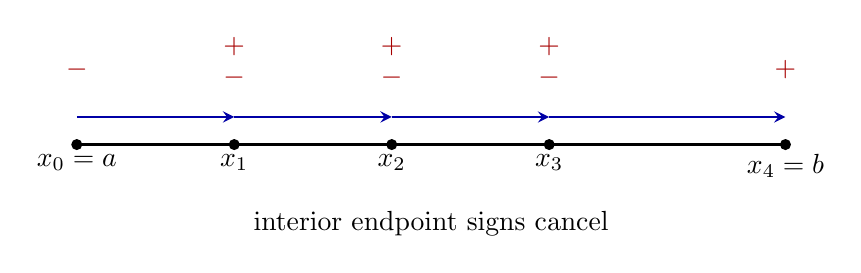
\begin{tikzpicture}[scale=1.0, >=stealth]
    \draw[thick] (0,0) -- (9,0);

    \foreach \x/\lab in {0/{x_0=a},2/{x_1},4/{x_2},6/{x_3},9/{x_4=b}} {
        \fill (\x,0) circle (2pt);
        \node[below] at (\x,0) {\(\lab\)};
    }

    \foreach \a/\b in {0/2,2/4,4/6,6/9} {
        \draw[->, thick, blue!65!black] (\a,0.35) -- (\b,0.35);
    }

    \node[red!65!black] at (2,0.85) {\(-\)};
    \node[red!65!black] at (2,1.25) {\(+\)};

    \node[red!65!black] at (4,0.85) {\(-\)};
    \node[red!65!black] at (4,1.25) {\(+\)};

    \node[red!65!black] at (6,0.85) {\(-\)};
    \node[red!65!black] at (6,1.25) {\(+\)};

    \node[red!65!black] at (0,0.95) {\(-\)};
    \node[red!65!black] at (9,0.95) {\(+\)};

    \node at (4.5,-1.0) {interior endpoint signs cancel};
\end{tikzpicture}
\caption{The one-dimensional cancellation behind the Fundamental Theorem of Calculus.}
\end{figure}

This same cancellation will reappear in the plane.  Instead of interior endpoints, we
will have interior edges.  Instead of \(df\), we will have \(d(P\,dx+Q\,dy)\).

\subsection{Why the smoothness condition is not decorative}

The theorem asked for \(f\) to be \(C^1\).  That is stronger than just being a function
with endpoint values.  The derivative \(df\) must exist and behave well throughout the
interval.

Here is what can go wrong.

\begin{example}[A hidden jump breaks the naive formula]
Define
\[
    f(x)=
    \begin{cases}
    0, & x<0,\\
    1, & x\ge 0.
    \end{cases}
\]
on the interval
\[
    [-1,1].
\]
The boundary integral is
\[
    \int_{\partial[-1,1]}f=f(1)-f(-1)=1-0=1.
\]

Away from \(x=0\), the function is constant, so a careless person might say
\[
    df=0
\]
and conclude
\[
    \int_{[-1,1]}df=0.
\]
That would give
\[
    1=0,
\]
which is false.

The problem is the jump at \(x=0\).  The function is not continuous there, and it is not
\(C^1\).  In our rules, \(df\) is not a valid continuous \(1\)-form on the whole interval.
The theorem was never allowed to be used.

The missing smoothness is hiding an internal boundary.
\end{example}

A corner is less dangerous than a jump, but it still needs care.

\begin{example}[A corner can be handled by splitting]
Let
\[
    f(x)=|x|
\]
on
\[
    [-1,1].
\]
This function is continuous, but it is not differentiable at \(x=0\).  So the \(C^1\)
version of the theorem does not apply directly.

But if we split the interval into two smooth pieces,
\[
    [-1,0]
    \qquad\text{and}\qquad
    [0,1],
\]
then
\[
    f(x)=-x
    \quad\text{on }[-1,0],
\]
and
\[
    f(x)=x
    \quad\text{on }[0,1].
\]
Thus
\[
\begin{aligned}
    \int_{-1}^{0}(-1)\,dx+\int_0^1 1\,dx
    &=
    -1+1\\
    &=
    0.
\end{aligned}
\]
The endpoint difference is also
\[
    f(1)-f(-1)=1-1=0.
\]

The formula survives after splitting, because the function has no jump.  But the
single \(C^1\) theorem did not cover the whole interval at once.
\end{example}

This is a useful pattern.  Piecewise smooth objects are usually allowed, but the pieces
and their boundary signs must be accounted for honestly.

\subsection{The first Stokes theorem}

The Fundamental Theorem of Calculus is often introduced as a theorem about
antiderivatives.  In this chapter, it is better to see it as the first boundary theorem.

It says:

\[
\boxed{
    \text{the total derivative inside an interval equals the signed value on the boundary.}
}
\]

The phrase ``signed value on the boundary'' is the new part.  Once we learn to hear it,
the theorem no longer feels like a one-dimensional accident.

The interval has two boundary points.  A plane region has a boundary curve.  When the
same idea moves from endpoints to curves, the derivative inside changes from
\[
    df
\]
to
\[
    d(P\,dx+Q\,dy).
\]
That is where Green's theorem enters the story.

\section{Green's Theorem as Stokes}
\label{sec:18.4}

The previous section turned the Fundamental Theorem of Calculus into
\[
    \int_{\partial[a,b]}f=\int_{[a,b]}df.
\]
Now the object \(M\) becomes a plane region \(R\).  Its boundary is no longer two
endpoints.  It is a closed curve.

The form on the boundary is no longer a function.  It is a \(1\)-form:
\[
    \omega=P\,dx+Q\,dy.
\]
Its derivative is a \(2\)-form:
\[
    d\omega=(Q_x-P_y)\,dx\wedge dy.
\]

That is Green's theorem in Stokes form.

\subsection{A triangular region that measures area from its boundary}

Let \(R\) be the triangle with vertices
\[
    (0,0),\qquad (3,0),\qquad (0,2),
\]
oriented by the standard area form
\[
    dx\wedge dy.
\]
Then \(\partial R\) is walked counterclockwise.

Take the \(1\)-form
\[
    \omega=x\,dy.
\]
Its exterior derivative is
\[
    d\omega=dx\wedge dy.
\]
So the right-hand side of Stokes should be
\[
    \int_R dx\wedge dy=\operatorname{Area}(R)=3.
\]

Now compute the boundary integral directly.

The boundary has three sides.

\subsubsection*{Bottom side}

Parametrize the bottom edge by
\[
    \mathbf r_1(t)=(t,0),
    \qquad
    0\le t\le3.
\]
Here
\[
    dy=0,
\]
so
\[
    \int_{\mathbf r_1}x\,dy=0.
\]

\subsubsection*{Slanted side}

Parametrize the slanted side from \((3,0)\) to \((0,2)\) by
\[
    \mathbf r_2(t)=(3-3t,2t),
    \qquad
    0\le t\le1.
\]
Then
\[
    x=3-3t,
    \qquad
    dy=2\,dt.
\]
Therefore
\[
\begin{aligned}
    \int_{\mathbf r_2}x\,dy
    &=
    \int_0^1 (3-3t)\,2\,dt\\
    &=
    \int_0^1 (6-6t)\,dt\\
    &=
    3.
\end{aligned}
\]

\subsubsection*{Left side}

Parametrize the left side from \((0,2)\) back to \((0,0)\) by
\[
    \mathbf r_3(t)=(0,2-2t),
    \qquad
    0\le t\le1.
\]
Here
\[
    x=0,
\]
so
\[
    \int_{\mathbf r_3}x\,dy=0.
\]

Adding the three sides gives
\[
\boxed{
    \int_{\partial R}x\,dy=3.
}
\]
And the interior integral gives
\[
\boxed{
    \int_R d(x\,dy)=\int_R dx\wedge dy=3.
}
\]
Thus
\[
\boxed{
    \int_{\partial R}\omega=\int_R d\omega.
}
\]

\begin{figure}[h]
\centering
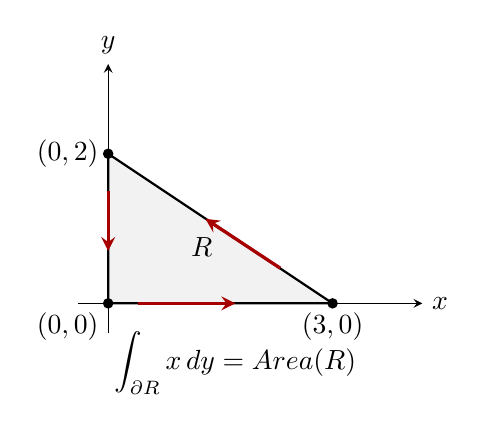
\begin{tikzpicture}[scale=0.95, >=stealth]
    \draw[->] (-0.4,0) -- (4.2,0) node[right] {\(x\)};
    \draw[->] (0,-0.4) -- (0,3.2) node[above] {\(y\)};

    \draw[fill=gray!10, thick] (0,0) -- (3,0) -- (0,2) -- cycle;

    \draw[->, very thick, red!65!black] (0.4,0) -- (1.7,0);
    \draw[->, very thick, red!65!black] (2.3,0.47) -- (1.3,1.13);
    \draw[->, very thick, red!65!black] (0,1.5) -- (0,0.7);

    \fill (0,0) circle (2pt);
    \fill (3,0) circle (2pt);
    \fill (0,2) circle (2pt);

    \node[below left] at (0,0) {\((0,0)\)};
    \node[below] at (3,0) {\((3,0)\)};
    \node[left] at (0,2) {\((0,2)\)};

    \node at (1.25,0.75) {\(R\)};
    \node at (1.7,-0.8) {\(\displaystyle \int_{\partial R}x\,dy=\operatorname{Area}(R)\)};
\end{tikzpicture}
\caption{For this triangle, the boundary integral of \(x\,dy\) measures area.}
\end{figure}

This example is Green's theorem in its cleanest form.  The boundary form \(x\,dy\)
turns into the area form \(dx\wedge dy\).

\subsection{Exterior derivative and scalar curl}

Let
\[
    \omega=P(x,y)\,dx+Q(x,y)\,dy
\]
be a \(1\)-form on a plane region.  To compute \(d\omega\), use
\[
    d(P\,dx)=dP\wedge dx,
\]
and
\[
    d(Q\,dy)=dQ\wedge dy.
\]
Since
\[
    dP=P_x\,dx+P_y\,dy,
\]
we get
\[
\begin{aligned}
    d(P\,dx)
    &=
    (P_x\,dx+P_y\,dy)\wedge dx\\
    &=
    P_x\,dx\wedge dx+P_y\,dy\wedge dx\\
    &=
    -P_y\,dx\wedge dy.
\end{aligned}
\]
Similarly,
\[
\begin{aligned}
    d(Q\,dy)
    &=
    (Q_x\,dx+Q_y\,dy)\wedge dy\\
    &=
    Q_x\,dx\wedge dy+Q_y\,dy\wedge dy\\
    &=
    Q_x\,dx\wedge dy.
\end{aligned}
\]
Therefore
\[
\boxed{
    d\omega=(Q_x-P_y)\,dx\wedge dy.
}
\]

The coefficient
\[
    Q_x-P_y
\]
is the scalar curl in the plane.  It measures local counterclockwise circulation per
unit area.

\[
\boxed{
    \text{exterior derivative of a plane }1\text{-form}
    =
    \text{scalar curl}\times\text{area form}.
}
\]

\subsection{Green's theorem in circulation form}

We can now read Green's theorem as one row of the generalized Stokes theorem.

\begin{theorem}[Green's theorem as Stokes]
Let \(R\) be a compact, oriented, piecewise smooth plane region.  Give
\(\partial R\) the positive boundary orientation, so that \(R\) stays on the left as the
boundary is traveled.

Let
\[
    \omega=P\,dx+Q\,dy
\]
be a \(C^1\) \(1\)-form on an open set containing \(R\).  Then
\[
\boxed{
    \int_{\partial R}\omega=\int_R d\omega.
}
\]
Equivalently,
\[
\boxed{
    \oint_{\partial R}P\,dx+Q\,dy
    =
    \iint_R (Q_x-P_y)\,dx\wedge dy.
}
\]
Using ordinary area notation,
\[
\boxed{
    \oint_{\partial R}P\,dx+Q\,dy
    =
    \iint_R (Q_x-P_y)\,dA.
}
\]
\end{theorem}

This is the same theorem students usually meet as Green's theorem.  The forms version
only makes the structure visible:
\[
    \omega
    \quad\text{lives on the boundary curve,}
\]
while
\[
    d\omega
    \quad\text{lives on the plane region.}
\]

\subsection{A rectangle with changing curl}

Let
\[
    R=[0,2]\times[0,1],
\]
with positive orientation, and let
\[
    \omega=xy\,dx+x^2\,dy.
\]
Then
\[
    P=xy,
    \qquad
    Q=x^2.
\]
So
\[
    P_y=x,
    \qquad
    Q_x=2x.
\]
Therefore
\[
    d\omega=(2x-x)\,dx\wedge dy=x\,dx\wedge dy.
\]

The interior integral is
\[
\begin{aligned}
    \int_R d\omega
    &=
    \int_0^2\int_0^1 x\,dy\,dx\\
    &=
    \int_0^2 x\,dx\\
    &=
    2.
\end{aligned}
\]

Now check the boundary integral.

On the bottom edge, \(y=0\) and \(dy=0\), so
\[
    \omega=0.
\]
The bottom contributes \(0\).

On the right edge, \(x=2\), \(dx=0\), and \(y\) goes from \(0\) to \(1\).  Thus
\[
    \omega=4\,dy,
\]
so the right edge contributes
\[
    \int_0^1 4\,dy=4.
\]

On the top edge, \(y=1\), \(dy=0\), and \(x\) goes from \(2\) back to \(0\).  Thus
\[
    \omega=x\,dx,
\]
so the top edge contributes
\[
    \int_2^0 x\,dx=-2.
\]

On the left edge, \(x=0\), so \(\omega=0\).  The left edge contributes \(0\).

Therefore
\[
\boxed{
    \int_{\partial R}\omega=4-2=2.
}
\]
Again,
\[
\boxed{
    \int_{\partial R}\omega=\int_R d\omega.
}
\]

\begin{figure}[h]
\centering
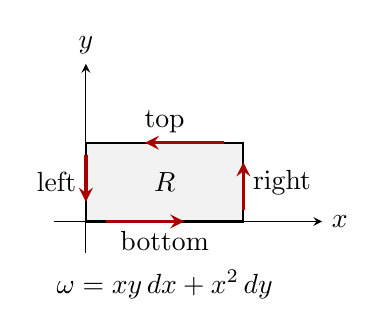
\begin{tikzpicture}[scale=1.0, >=stealth]
    \draw[->] (-0.4,0) -- (3.0,0) node[right] {\(x\)};
    \draw[->] (0,-0.4) -- (0,2.0) node[above] {\(y\)};

    \draw[fill=gray!10, thick] (0,0) rectangle (2,1);

    \draw[->, very thick, red!65!black] (0.25,0) -- (1.25,0);
    \draw[->, very thick, red!65!black] (2,0.15) -- (2,0.75);
    \draw[->, very thick, red!65!black] (1.75,1) -- (0.75,1);
    \draw[->, very thick, red!65!black] (0,0.85) -- (0,0.25);

    \node[below] at (1,0) {bottom};
    \node[right] at (2,0.5) {right};
    \node[above] at (1,1) {top};
    \node[left] at (0,0.5) {left};

    \node at (1,0.5) {\(R\)};
    \node at (1,-0.8) {\(\omega=xy\,dx+x^2\,dy\)};
\end{tikzpicture}
\caption{The boundary contributions add to the integral of \(d\omega=x\,dx\wedge dy\)
inside the rectangle.}
\end{figure}

\subsection{Why interior edges cancel}

The proof idea is the same as in one dimension.

Cut \(R\) into many small rectangles.  Apply Green's theorem on each small rectangle.
Now add all the small boundary integrals.

Every interior edge is traveled twice:
\[
    \text{once in one direction, once in the opposite direction.}
\]
A \(1\)-form integral changes sign when the direction reverses.  So the two
contributions cancel.

Only the outer boundary remains.

\[
\boxed{
    \text{interior edges cancel; exterior edges survive.}
}
\]

That is the same cancellation we saw for an interval, where interior endpoints canceled.
Green's theorem is the two-dimensional version of the same boundary bookkeeping.

\subsection{Holes and boundary components}

If a region has a hole, the boundary has more than one component.  Green's theorem
uses all of them.

The outer boundary is counterclockwise.  The inner boundary is clockwise.

Here is a compact example that shows why.

Let
\[
    A=\{(x,y):1\le x^2+y^2\le4\}
\]
be the annulus between the circles of radius \(1\) and \(2\).  Consider the \(1\)-form
\[
    \alpha=
    \frac{-y}{x^2+y^2}\,dx+
    \frac{x}{x^2+y^2}\,dy.
\]
This form is defined on the annulus, because the origin is not included.  On that
domain,
\[
    d\alpha=0.
\]
So Green's theorem predicts
\[
    \int_{\partial A}\alpha=0.
\]

Now compute the boundary.  On a counterclockwise circle of radius \(r\),
\[
    x=r\cos t,
    \qquad
    y=r\sin t,
    \qquad
    0\le t\le2\pi.
\]
Then
\[
    dx=-r\sin t\,dt,
    \qquad
    dy=r\cos t\,dt.
\]
Substitute:
\[
\begin{aligned}
    \alpha
    &=
    \frac{-r\sin t}{r^2}(-r\sin t\,dt)
    +
    \frac{r\cos t}{r^2}(r\cos t\,dt)\\
    &=
    \sin^2t\,dt+\cos^2t\,dt\\
    &=
    dt.
\end{aligned}
\]
So a counterclockwise circle contributes
\[
    \int_0^{2\pi}dt=2\pi.
\]

The outer boundary of the annulus is counterclockwise, so it contributes
\[
    2\pi.
\]
The inner boundary is clockwise, so it contributes
\[
    -2\pi.
\]
Thus
\[
\boxed{
    \int_{\partial A}\alpha=2\pi-2\pi=0,
}
\]
which matches
\[
    \int_A d\alpha=0.
\]

If we forgot the inner boundary, we would get \(2\pi\), which would contradict the
theorem.  The theorem did not fail.  The boundary was incomplete.

\subsection{A singularity inside the region is not allowed}

The same form
\[
    \alpha=
    \frac{-y}{x^2+y^2}\,dx+
    \frac{x}{x^2+y^2}\,dy
\]
is closed wherever it is defined:
\[
    d\alpha=0
    \qquad
    \text{on }\mathbb R^2\setminus\{(0,0)\}.
\]

But on the unit circle,
\[
    \int_{x^2+y^2=1}\alpha=2\pi.
\]
A careless person might try to apply Green's theorem to the unit disk and say
\[
    \int_{\partial D}\alpha
    =
    \int_D d\alpha
    =
    0.
\]
That is not allowed.  The form is not defined at the origin, and the origin lies inside
the disk.

The missing point is exactly what the boundary circle detects.

\[
\boxed{
    \text{Green's theorem requires the form to be defined on the whole region, not only on the boundary.}
}
\]

\subsection{A jump in the coefficients creates a hidden edge}

The \(C^1\) condition on \(P\) and \(Q\) also matters.  If the coefficients jump, the
usual formula can miss an internal boundary.

Let
\[
    R=[-1,1]\times[-1,1],
\]
and define
\[
    H(y)=
    \begin{cases}
    0, & y<0,\\
    1, & y>0.
    \end{cases}
\]
Consider the form
\[
    \omega=H(y)\,dx.
\]
This form jumps across the line \(y=0\), so it is not \(C^1\) on \(R\).

If we ignore the jump and only look away from \(y=0\), then \(H\) is constant on each
side, so a careless computation would say
\[
    d\omega=0.
\]
That would predict
\[
    \int_{\partial R}\omega=0.
\]

But the boundary integral is not zero.  On the bottom edge \(y=-1\),
\[
    H(y)=0,
\]
so the bottom contributes \(0\).  On the top edge \(y=1\), the boundary is traveled
from \(x=1\) to \(x=-1\), and
\[
    H(y)=1.
\]
So the top contributes
\[
    \int_1^{-1} dx=-2.
\]
The vertical sides have \(dx=0\).  Hence
\[
\boxed{
    \int_{\partial R}\omega=-2.
}
\]

The jump along \(y=0\) is hiding an internal edge.  The ordinary \(C^1\) theorem is
not designed to handle it.

\subsection{Flux form of Green's theorem}

Green's theorem also has a flux version.

Let
\[
    \mathbf F=(A,B)
\]
be a vector field in the plane.  The outward flux of \(\mathbf F\) across a positively
oriented boundary is represented by the \(1\)-form
\[
\boxed{
    \phi=A\,dy-B\,dx.
}
\]

To see why, parametrize the boundary by
\[
    \mathbf r(t)=(x(t),y(t))
\]
in positive orientation.  Then the tangent direction keeps the region on the left, so the
outward normal points to the right.  A right normal times \(ds\) is
\[
    (dy,-dx).
\]
Therefore
\[
    \mathbf F\cdot\mathbf n_{\text{out}}\,ds
    =
    (A,B)\cdot(dy,-dx)
    =
    A\,dy-B\,dx.
\]

Now compute the exterior derivative:
\[
\begin{aligned}
    d\phi
    &=
    d(A\,dy-B\,dx)\\
    &=
    dA\wedge dy-dB\wedge dx\\
    &=
    A_x\,dx\wedge dy+B_y\,dx\wedge dy\\
    &=
    (A_x+B_y)\,dx\wedge dy.
\end{aligned}
\]
The coefficient
\[
    A_x+B_y
\]
is the divergence of \(\mathbf F\).

So Green's theorem becomes
\[
\boxed{
    \int_{\partial R} A\,dy-B\,dx
    =
    \int_R (A_x+B_y)\,dx\wedge dy.
}
\]
In vector notation,
\[
\boxed{
    \oint_{\partial R}\mathbf F\cdot\mathbf n_{\text{out}}\,ds
    =
    \iint_R \nabla\cdot\mathbf F\,dA.
}
\]

This is the two-dimensional divergence theorem.

\begin{example}[Flux out of a circular pond]
Let
\[
    \mathbf F(x,y)=(x,y),
\]
the radial field pointing away from the origin.  The flux form is
\[
    \phi=x\,dy-y\,dx.
\]
Its exterior derivative is
\[
    d\phi=2\,dx\wedge dy.
\]

Let \(D_a\) be the disk of radius \(a\).  The interior integral is
\[
    \int_{D_a}2\,dx\wedge dy=2\pi a^2.
\]

Now compute the boundary flux directly.  Parametrize the boundary circle
counterclockwise:
\[
    x=a\cos t,
    \qquad
    y=a\sin t,
    \qquad
    0\le t\le2\pi.
\]
Then
\[
    dx=-a\sin t\,dt,
    \qquad
    dy=a\cos t\,dt.
\]
So
\[
\begin{aligned}
    x\,dy-y\,dx
    &=
    (a\cos t)(a\cos t\,dt)
    -
    (a\sin t)(-a\sin t\,dt)\\
    &=
    a^2(\cos^2t+\sin^2t)\,dt\\
    &=
    a^2\,dt.
\end{aligned}
\]
Thus
\[
    \int_{\partial D_a}\phi
    =
    \int_0^{2\pi}a^2\,dt
    =
    2\pi a^2.
\]
Again,
\[
\boxed{
    \int_{\partial D_a}\phi=\int_{D_a}d\phi.
}
\]
\end{example}

\subsection{Two Green's theorems, one Stokes theorem}

The circulation form of Green's theorem uses
\[
    \omega=P\,dx+Q\,dy.
\]
It gives
\[
\boxed{
    \oint_{\partial R}P\,dx+Q\,dy
    =
    \iint_R (Q_x-P_y)\,dA.
}
\]

The flux form uses
\[
    \phi=A\,dy-B\,dx.
\]
It gives
\[
\boxed{
    \oint_{\partial R}\mathbf F\cdot\mathbf n_{\text{out}}\,ds
    =
    \iint_R \nabla\cdot\mathbf F\,dA.
}
\]

They look like two different vector calculus formulas.  In forms language, they are the
same theorem:
\[
\boxed{
    \int_{\partial R}\text{form}=\int_R d(\text{form}).
}
\]

The only difference is which \(1\)-form we choose for the boundary measurement.

Green's theorem is Stokes' theorem on a flat surface.  But a boundary curve in space
does not have to lie flat.  A wire loop can bend and twist, and a soap film can stretch
across it in many possible shapes.  The boundary is still a curve, but the inside is now
a surface.  The next disguise of the same theorem is the one that carries curl from a
flat region into space.

\section{Classical Stokes' theorem as generalized Stokes}
\label{sec:18.5}

Section \ref{sec:18.4} kept everything flat.  A plane region \(R\) had a boundary
curve \(\partial R\), and Green's theorem became
\[
    \int_{\partial R}\omega=\int_R d\omega.
\]
Now the region is allowed to bend into space.  The boundary is still a curve, but the
inside is a surface.

This is classical Stokes' theorem.

\subsection{A tilted sheet and a boundary integral}

Start with a tilted rectangular sheet in space:
\[
    \mathbf r(u,v)=(u,v,u+2v),
    \qquad
    0\le u\le2,\quad 0\le v\le1.
\]
The parameter rectangle is
\[
    D=[0,2]\times[0,1].
\]
The surface orientation is determined by
\[
    \mathbf r_u\times\mathbf r_v.
\]
Since
\[
    \mathbf r_u=(1,0,1),
    \qquad
    \mathbf r_v=(0,1,2),
\]
we get
\[
    \mathbf r_u\times\mathbf r_v=(-1,-2,1).
\]

Now take the \(1\)-form
\[
    \omega=z\,dy.
\]
This form is built to be integrated along the boundary curve of the tilted sheet.

Instead of parametrizing the four boundary curves directly in space, pull the form back
to the parameter rectangle.  On the surface,
\[
    x=u,\qquad y=v,\qquad z=u+2v.
\]
So
\[
    dy=dv,
\]
and
\[
    \mathbf r^*\omega=(u+2v)\,dv.
\]

The boundary of \(D\) is positively oriented counterclockwise.  Compute the integral
around its four sides.

On the bottom side \(v=0\), \(dv=0\), so the contribution is \(0\).

On the right side \(u=2\), \(v\) goes from \(0\) to \(1\), so
\[
    \int_{\text{right}}(u+2v)\,dv
    =
    \int_0^1(2+2v)\,dv
    =
    3.
\]

On the top side \(v=1\), \(dv=0\), so the contribution is \(0\).

On the left side \(u=0\), \(v\) goes from \(1\) down to \(0\), so
\[
    \int_{\text{left}}(u+2v)\,dv
    =
    \int_1^0 2v\,dv
    =
    -1.
\]

Adding the four sides gives
\[
\boxed{
    \int_{\partial S}\omega
    =
    \int_{\partial D}\mathbf r^*\omega
    =
    3-1
    =
    2.
}
\]

Now compute the surface side.  Since
\[
    \omega=z\,dy,
\]
we have
\[
    d\omega=dz\wedge dy.
\]
Pull this back:
\[
    dz=d(u+2v)=du+2\,dv,
\]
so
\[
\begin{aligned}
    \mathbf r^*(d\omega)
    &=
    (du+2\,dv)\wedge dv\\
    &=
    du\wedge dv.
\end{aligned}
\]
Therefore
\[
\begin{aligned}
    \int_S d\omega
    &=
    \int_D \mathbf r^*(d\omega)\\
    &=
    \int_D du\wedge dv\\
    &=
    \operatorname{Area}(D)\\
    &=
    2.
\end{aligned}
\]
So
\[
\boxed{
    \int_{\partial S}\omega=\int_S d\omega.
}
\]


\begin{figure}[h]
\centering
\begin{tikzpicture}[scale=0.82, >=stealth]
    \begin{scope}
        \draw[->] (-0.35,0) -- (3.1,0) node[right] {\(u\)};
        \draw[->] (0,-0.35) -- (0,2.25) node[above] {\(v\)};

        \draw[fill=gray!10, thick] (0,0) rectangle (2.4,1.4);

        \draw[->, very thick, red!65!black] (0,0) -- (1.0,0);
        \draw[->, very thick, red!65!black] (2.4,0) -- (2.4,0.75);
        \draw[->, very thick, red!65!black] (2.4,1.4) -- (1.4,1.4);
        \draw[->, very thick, red!65!black] (0,1.4) -- (0,0.65);

        \node at (1.2,-0.75) {parameter rectangle \(D\)};
    \end{scope}

    \draw[->, thick] (3.4,0.75) -- (4.8,0.75);
    \node[above] at (4.1,0.75) {\(\mathbf r\)};

    \begin{scope}[shift={(6.1,-0.1)}]
        \coordinate (A) at (0,0);
        \coordinate (B) at (3.1,0.45);
        \coordinate (C) at (3.55,1.75);
        \coordinate (D) at (0.45,1.30);

        \draw[fill=blue!7, thick] (A)--(B)--(C)--(D)--cycle;

        \draw[->, very thick, red!65!black] (A)--($(A)!0.42!(B)$);
        \draw[->, very thick, red!65!black] (B)--($(B)!0.55!(C)$);
        \draw[->, very thick, red!65!black] (C)--($(C)!0.42!(D)$);
        \draw[->, very thick, red!65!black] (D)--($(D)!0.55!(A)$);

        % The vector now correctly points up and out, governed by the right-hand rule
        \draw[->, very thick, blue!65!black] (1.8,0.8) -- ++(-0.4, 1.4)
            node[above] {\(\mathbf r_u\times\mathbf r_v\)};

        \node at (1.85,-0.95) {tilted surface \(S\)};
    \end{scope}
\end{tikzpicture}
\caption{A positively oriented parameter rectangle induces the compatible orientation on
the boundary of the surface.}
\end{figure}

The computation contains the whole theorem.  The boundary integral on the surface was
turned into a boundary integral on the parameter rectangle.  Then Green's theorem took
over.

\subsection{Pullback to a parameter domain}

A parametrized surface
\[
    \mathbf r(u,v)=(x(u,v),y(u,v),z(u,v))
\]
lets us translate forms in space into forms in the parameter plane.

For a \(1\)-form
\[
    \omega=P\,dx+Q\,dy+R\,dz,
\]
the pullback is
\[
\boxed{
    \mathbf r^*\omega
    =
    P(\mathbf r(u,v))\,d x(u,v)
    +
    Q(\mathbf r(u,v))\,d y(u,v)
    +
    R(\mathbf r(u,v))\,d z(u,v).
}
\]
Here
\[
    dx=x_u\,du+x_v\,dv,
\]
\[
    dy=y_u\,du+y_v\,dv,
\]
and
\[
    dz=z_u\,du+z_v\,dv.
\]

The pullback does two jobs at once.  It substitutes the parametrization into the
coefficients, and it replaces \(dx,dy,dz\) by the coordinate changes caused by \(du\)
and \(dv\).

For integrals, the rule is
\[
\boxed{
    \int_S \alpha=\int_D \mathbf r^*\alpha,
}
\]
when \(\alpha\) is a form of degree \(2\) on the surface.

For boundary integrals,
\[
\boxed{
    \int_{\partial S}\omega=\int_{\partial D}\mathbf r^*\omega,
}
\]
provided the boundary orientation on \(S\) is induced from the boundary orientation
on \(D\).

The most important identity is
\[
\boxed{
    d(\mathbf r^*\omega)=\mathbf r^*(d\omega).
}
\]
This is the chain rule in form language.  It says that pulling back and differentiating
fit together.

Now apply Green's theorem on \(D\):
\[
    \int_{\partial D}\mathbf r^*\omega
    =
    \int_D d(\mathbf r^*\omega).
\]
Using
\[
    d(\mathbf r^*\omega)=\mathbf r^*(d\omega),
\]
we get
\[
    \int_{\partial D}\mathbf r^*\omega
    =
    \int_D \mathbf r^*(d\omega).
\]
Translated back to the surface, this becomes
\[
    \int_{\partial S}\omega=\int_S d\omega.
\]

That is Stokes' theorem.

\subsection{Curl as the exterior derivative of a \(1\)-form}

Let
\[
    \mathbf F=(P,Q,R)
\]
be a vector field, and let
\[
    \omega=P\,dx+Q\,dy+R\,dz
\]
be its work \(1\)-form.

Compute \(d\omega\):
\[
\begin{aligned}
d\omega
&=
dP\wedge dx+dQ\wedge dy+dR\wedge dz\\
&=
(R_y-Q_z)\,dy\wedge dz\\
&\quad+
(P_z-R_x)\,dz\wedge dx\\
&\quad+
(Q_x-P_y)\,dx\wedge dy.
\end{aligned}
\]

The coefficients are exactly the components of the curl:
\[
\boxed{
    \nabla\times\mathbf F
    =
    (R_y-Q_z,\;P_z-R_x,\;Q_x-P_y).
}
\]
So
\[
\boxed{
    d\omega=\Phi_{\nabla\times\mathbf F},
}
\]
where
\[
    \Phi_{\nabla\times\mathbf F}
\]
is the flux \(2\)-form of the vector field \(\nabla\times\mathbf F\).

In words:
\[
\boxed{
    \text{the exterior derivative of the work form is the flux form of the curl.}
}
\]

This is why the right side of classical Stokes' theorem contains curl.

\subsection{Boundary circulation equals surface curl}

Now the theorem can be written in both languages.

\begin{theorem}[Classical Stokes' theorem as generalized Stokes]
Let \(S\) be an oriented compact piecewise smooth surface in space, with piecewise
smooth boundary \(\partial S\).  Give \(\partial S\) the boundary orientation compatible
with the orientation of \(S\).

Let
\[
    \omega=P\,dx+Q\,dy+R\,dz
\]
be a \(C^1\) \(1\)-form on an open set containing \(S\).  Then
\[
\boxed{
    \int_{\partial S}\omega=\int_S d\omega.
}
\]

Equivalently, for the vector field
\[
    \mathbf F=(P,Q,R),
\]
\[
\boxed{
    \oint_{\partial S}\mathbf F\cdot d\mathbf r
    =
    \iint_S(\nabla\times\mathbf F)\cdot \widehat{\mathbf n}\,dS.
}
\]
\end{theorem}

The forms statement is the generalized Stokes theorem with
\[
    M=S,
    \qquad
    \omega\text{ a }1\text{-form}.
\]
The vector statement is the classical formula students often learn first.

The left side is boundary circulation.  The right side is curl passing through the
surface.

\subsection{A curved surface with the same boundary}

Let
\[
    \omega=-\frac y2\,dx+\frac x2\,dy.
\]
Then
\[
    d\omega=dx\wedge dy.
\]

Let \(S\) be the upper hemisphere
\[
    x^2+y^2+z^2=a^2,
    \qquad z\ge0,
\]
oriented by the upward/outward normal.  Its boundary is the circle
\[
    C:\quad x^2+y^2=a^2,\qquad z=0,
\]
oriented counterclockwise as viewed from above.

Compute the boundary integral.  Parametrize \(C\) by
\[
    x=a\cos t,\qquad y=a\sin t,\qquad z=0,
    \qquad 0\le t\le2\pi.
\]
Then
\[
    dx=-a\sin t\,dt,
    \qquad
    dy=a\cos t\,dt.
\]
So
\[
\begin{aligned}
    \omega
    &=
    -\frac{a\sin t}{2}(-a\sin t\,dt)
    +
    \frac{a\cos t}{2}(a\cos t\,dt)\\
    &=
    \frac{a^2}{2}(\sin^2 t+\cos^2 t)\,dt\\
    &=
    \frac{a^2}{2}\,dt.
\end{aligned}
\]
Thus
\[
\boxed{
    \int_C\omega=\pi a^2.
}
\]

Now compute the surface integral.  Since
\[
    d\omega=dx\wedge dy,
\]
the integral
\[
    \int_S dx\wedge dy
\]
measures the signed area of the shadow of \(S\) on the \(xy\)-plane.  With upward
orientation, that shadow is the disk
\[
    x^2+y^2\le a^2
\]
with positive orientation.  Therefore
\[
\boxed{
    \int_S d\omega=\int_S dx\wedge dy=\pi a^2.
}
\]
Again,
\[
\boxed{
    \int_{\partial S}\omega=\int_S d\omega.
}
\]

The hemisphere and the flat disk have the same boundary.  For this form, both surfaces
give the same answer because Stokes' theorem only sees the boundary.

\subsection{Why the hypotheses matter}

Stokes' theorem is a sign-sensitive theorem.  It is also sensitive to holes and
singularities.

\subsubsection*{The boundary orientation must be compatible}

Use the disk
\[
    x^2+y^2\le1,\qquad z=0,
\]
with upward orientation, and use
\[
    \omega=-\frac y2\,dx+\frac x2\,dy.
\]
Then
\[
    d\omega=dx\wedge dy,
\]
so
\[
    \int_S d\omega=\pi.
\]

The compatible boundary orientation is counterclockwise.  With that orientation,
\[
    \int_{\partial S}\omega=\pi.
\]

If we walk the same boundary clockwise, the boundary integral becomes
\[
    -\pi.
\]
The surface integral has not changed.  The problem is not the theorem; the boundary
orientation was wrong.

\subsubsection*{Every boundary component must be included}

Let
\[
    A=\{(x,y,0):1\le x^2+y^2\le4\}
\]
be a flat annulus with upward orientation.  Its boundary has two components:
\[
    C_{\text{outer}}:\ x^2+y^2=4,
\]
and
\[
    C_{\text{inner}}:\ x^2+y^2=1.
\]
The compatible orientation is counterclockwise on the outer circle and clockwise on the
inner circle.

For
\[
    \omega=-\frac y2\,dx+\frac x2\,dy,
\]
we have
\[
    d\omega=dx\wedge dy.
\]
Therefore
\[
    \int_A d\omega=\operatorname{Area}(A)=4\pi-\pi=3\pi.
\]

On a counterclockwise circle of radius \(r\),
\[
    \int\omega=\pi r^2.
\]
So the outer boundary contributes
\[
    4\pi,
\]
while the clockwise inner boundary contributes
\[
    -\pi.
\]
Thus
\[
    \int_{\partial A}\omega=4\pi-\pi=3\pi.
\]

If we forgot the inner boundary, the left side would be \(4\pi\), not \(3\pi\).
The hole has a rim, and Stokes' theorem counts that rim with its induced sign.

\subsubsection*{The form must be defined on the whole surface}

Consider
\[
    \alpha=
    -\frac{y}{x^2+y^2}\,dx
    +
    \frac{x}{x^2+y^2}\,dy.
\]
This form is defined away from the \(z\)-axis.  Where it is defined,
\[
    d\alpha=0.
\]

On the unit circle in the plane \(z=0\),
\[
    x=\cos t,\qquad y=\sin t,
\]
so
\[
    dx=-\sin t\,dt,\qquad dy=\cos t\,dt.
\]
Then
\[
\begin{aligned}
    \alpha
    &=
    -\sin t(-\sin t\,dt)+\cos t(\cos t\,dt)\\
    &=
    dt.
\end{aligned}
\]
Therefore
\[
\boxed{
    \int_C\alpha=2\pi.
}
\]

A careless use of Stokes' theorem on the flat unit disk would say
\[
    \int_C\alpha=\int_D d\alpha=0.
\]
But the form is not defined at the origin, and the origin lies in the disk.  Stokes'
theorem cannot be used there.

If we remove a small disk around the origin, the theorem works again.  The new surface
is an annulus.  Its outer boundary contributes \(2\pi\), and its inner boundary
contributes \(-2\pi\).  The total boundary integral is \(0\), matching
\[
    \int d\alpha=0
\]
on the annulus.

The missing point was not harmless.  It carried the circulation.

Stokes' theorem compares a boundary curve with a surface.  But some surfaces have no
boundary curve at all.  A sphere has no rim.  A closed box surface has no edge.  Still,
flux can pass through them.  To read that situation as Stokes' theorem, the object
inside must be one dimension higher: a solid region, with a \(2\)-form on its boundary.

\section{The divergence theorem as generalized Stokes}
\label{sec:18.6}

Section \ref{sec:18.5} used
\[
    M=S,
\]
where \(S\) was a surface and \(\partial S\) was a curve.  A \(1\)-form lived on the
boundary curve, and its exterior derivative lived on the surface:
\[
    \int_{\partial S}\omega=\int_S d\omega.
\]

Now move up one dimension.  Let
\[
    M=E
\]
be a solid region.  Its boundary is a surface.  So the boundary integrand must be a
\(2\)-form.

That is the divergence theorem.

\subsection{A \(2\)-form on a box}

Let
\[
    E=[0,2]\times[0,1]\times[0,3]
\]
with the standard orientation
\[
    dx\wedge dy\wedge dz.
\]
The boundary \(\partial E\) is oriented outward.

Take the \(2\)-form
\[
\boxed{
    \Phi=x\,dy\wedge dz+y\,dz\wedge dx+z\,dx\wedge dy.
}
\]
This is the flux \(2\)-form of the vector field
\[
    \mathbf F=(x,y,z).
\]

Compute the boundary integral face by face.

On the face \(x=2\), the outward normal is \(\mathbf i\), and the positive surface form is
\[
    dy\wedge dz.
\]
There,
\[
    x=2,
\]
so the contribution is
\[
    \int_{x=2}2\,dy\wedge dz=2(1)(3)=6.
\]

On the face \(x=0\), the coefficient \(x\) is zero, so the contribution is
\[
    0.
\]

On the face \(y=1\), the outward normal is \(\mathbf j\), and the positive surface form is
\[
    dz\wedge dx.
\]
There,
\[
    y=1,
\]
so the contribution is
\[
    \int_{y=1}1\,dz\wedge dx=1(3)(2)=6.
\]

On the face \(y=0\), the contribution is
\[
    0.
\]

On the face \(z=3\), the outward normal is \(\mathbf k\), and the positive surface form is
\[
    dx\wedge dy.
\]
There,
\[
    z=3,
\]
so the contribution is
\[
    \int_{z=3}3\,dx\wedge dy=3(2)(1)=6.
\]

On the face \(z=0\), the contribution is
\[
    0.
\]

Adding the six faces gives
\[
\boxed{
    \int_{\partial E}\Phi=6+6+6=18.
}
\]

Now compute the interior side.  Since
\[
    \Phi=x\,dy\wedge dz+y\,dz\wedge dx+z\,dx\wedge dy,
\]
we have
\[
\begin{aligned}
    d\Phi
    &=
    dx\wedge dy\wedge dz
    +
    dy\wedge dz\wedge dx
    +
    dz\wedge dx\wedge dy\\
    &=
    3\,dx\wedge dy\wedge dz.
\end{aligned}
\]
Therefore
\[
\begin{aligned}
    \int_E d\Phi
    &=
    \int_E 3\,dx\wedge dy\wedge dz\\
    &=
    3\operatorname{Volume}(E)\\
    &=
    3(2)(1)(3)\\
    &=
    18.
\end{aligned}
\]
So
\[
\boxed{
    \int_{\partial E}\Phi=\int_E d\Phi.
}
\]

\begin{figure}[h]
\centering
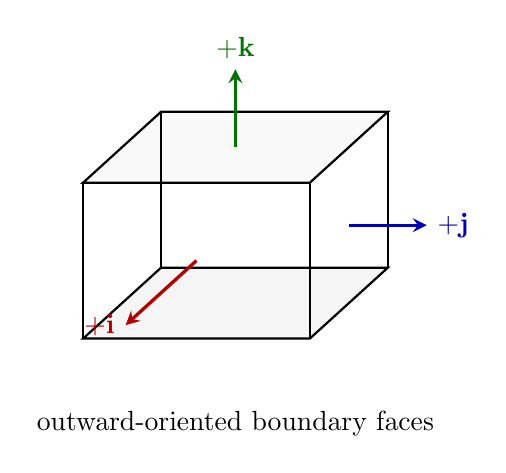
\begin{tikzpicture}[scale=0.9, >=stealth]
    % Coordinates for the box
    \coordinate (O) at (0,0);
    \coordinate (A) at (3.2,0);
    \coordinate (B) at (4.3,1.0);
    \coordinate (C) at (1.1,1.0);
    \coordinate (D) at (0,2.2);
    \coordinate (E) at (3.2,2.2);
    \coordinate (F) at (4.3,3.2);
    \coordinate (G) at (1.1,3.2);

    % Draw the box
    \draw[fill=gray!8, thick] (O)--(A)--(B)--(C)--cycle;
    \draw[fill=gray!5, thick] (D)--(E)--(F)--(G)--cycle;
    \draw[thick] (O)--(D);
    \draw[thick] (A)--(E);
    \draw[thick] (B)--(F);
    \draw[thick] (C)--(G);

    % +i direction: Center of the front face (O-A-E-D)
    % Center = (1.6, 1.1). Points out of the page (down-left).
    \draw[->, very thick, red!70!black] (1.6,1.1) -- (0.6,0.19) 
        node[left] {\(+\mathbf{i}\)};

    % +j direction: Center of the right face (A-B-F-E)
    % Center = (3.75, 1.6). Points right.
    \draw[->, very thick, blue!70!black] (3.75,1.6) -- (4.85,1.6) 
        node[right] {\(+\mathbf{j}\)};

    % +k direction: Center of the top face (D-E-F-G)
    % Center = (2.15, 2.7). Points up.
    \draw[->, very thick, green!45!black] (2.15,2.7) -- (2.15,3.8) 
        node[above] {\(+\mathbf{k}\)};

    \node at (2.15,-1.2) {outward-oriented boundary faces};
\end{tikzpicture}
\caption{For a solid, the boundary is a surface. A \(2\)-form is the correct boundary integrand.}
\end{figure}

The example has the same shape as every version of Stokes:
\[
    \text{form on the boundary}
    \qquad\longleftrightarrow\qquad
    \text{derivative of the form inside}.
\]

\subsection{Exterior derivative and divergence}

Let
\[
    \mathbf F=(P,Q,R)
\]
be a vector field in space.  Its flux \(2\)-form is
\[
\boxed{
    \Phi_{\mathbf F}
    =
    P\,dy\wedge dz
    +
    Q\,dz\wedge dx
    +
    R\,dx\wedge dy.
}
\]
Taking the exterior derivative gives
\[
\begin{aligned}
d\Phi_{\mathbf F}
&=
dP\wedge dy\wedge dz
+
dQ\wedge dz\wedge dx
+
dR\wedge dx\wedge dy\\
&=
P_x\,dx\wedge dy\wedge dz\\
&\quad+
Q_y\,dy\wedge dz\wedge dx\\
&\quad+
R_z\,dz\wedge dx\wedge dy\\
&=
(P_x+Q_y+R_z)\,dx\wedge dy\wedge dz.
\end{aligned}
\]
The coefficient is the divergence:
\[
\boxed{
    \nabla\cdot\mathbf F=P_x+Q_y+R_z.
}
\]
So
\[
\boxed{
    d\Phi_{\mathbf F}
    =
    (\nabla\cdot\mathbf F)\,dx\wedge dy\wedge dz.
}
\]

In words:
\[
\boxed{
    \text{the exterior derivative of the flux form is the divergence volume form.}
}
\]

A \(2\)-form measures oriented surface pieces.  Its derivative is a \(3\)-form, which
measures oriented volume pieces.  That is exactly the movement from boundary flux to
interior source.

\subsection{Boundary flux equals interior source}

The divergence theorem is the generalized Stokes theorem in dimension \(3\).

\begin{theorem}[Divergence theorem as generalized Stokes]
Let \(E\) be an oriented compact solid region in space with piecewise smooth boundary
\(\partial E\).  Give \(\partial E\) the outward boundary orientation.

Let
\[
    \Phi=P\,dy\wedge dz+Q\,dz\wedge dx+R\,dx\wedge dy
\]
be a \(C^1\) \(2\)-form on an open set containing \(E\).  Then
\[
\boxed{
    \int_{\partial E}\Phi=\int_E d\Phi.
}
\]

Equivalently, for the vector field
\[
    \mathbf F=(P,Q,R),
\]
\[
\boxed{
    \iint_{\partial E}\mathbf F\cdot\widehat{\mathbf n}_{\mathrm{out}}\,dS
    =
    \iiint_E \nabla\cdot\mathbf F\,dV.
}
\]
\end{theorem}

The forms statement is
\[
    \int_{\partial M}\omega=\int_M d\omega
\]
with
\[
    M=E,
    \qquad
    \omega=\Phi.
\]

The vector statement says:
\[
\boxed{
    \text{net outward flux through the boundary}
    =
    \text{total source strength inside}.
}
\]

\subsection{Flux out of a spherical tank}

Let \(E\) be the ball of radius \(a\) centered at the origin:
\[
    x^2+y^2+z^2\le a^2.
\]
Let
\[
    \mathbf F=(x,y,z),
\]
with flux form
\[
    \Phi=x\,dy\wedge dz+y\,dz\wedge dx+z\,dx\wedge dy.
\]
As above,
\[
    d\Phi=3\,dx\wedge dy\wedge dz.
\]
Therefore
\[
\begin{aligned}
    \int_{\partial E}\Phi
    &=
    \int_E d\Phi\\
    &=
    \int_E 3\,dx\wedge dy\wedge dz\\
    &=
    3\operatorname{Volume}(E)\\
    &=
    3\left(\frac43\pi a^3\right)\\
    &=
    4\pi a^3.
\end{aligned}
\]
So
\[
\boxed{
    \iint_{\partial E}(x,y,z)\cdot\widehat{\mathbf n}_{\mathrm{out}}\,dS
    =
    4\pi a^3.
}
\]

The direct surface calculation says the same thing.  On the sphere,
\[
    \widehat{\mathbf n}_{\mathrm{out}}=\frac{(x,y,z)}{a}.
\]
Thus
\[
    (x,y,z)\cdot\widehat{\mathbf n}_{\mathrm{out}}
    =
    \frac{x^2+y^2+z^2}{a}
    =
    a.
\]
So the outward flux is
\[
    a\cdot 4\pi a^2=4\pi a^3.
\]

The divergence theorem turned a surface integral into the volume of the ball.  The
surface was curved, but the interior source density was constant:
\[
    \nabla\cdot(x,y,z)=3.
\]

\subsection{Why the hypotheses matter}

The divergence theorem is often misused in three ways: the surface is not closed, the
orientation is not outward, or the field is not defined inside.  A fourth warning is
smoothness: jumps can hide internal sources.

\subsubsection*{The boundary surface must be closed}

Let \(D\) be the unit disk
\[
    x^2+y^2\le1,
    \qquad
    z=0,
\]
oriented upward.  Take the constant field
\[
    \mathbf F=(0,0,1),
\]
with flux form
\[
    \Phi=dx\wedge dy.
\]
Then
\[
    \int_D\Phi=\pi.
\]
But
\[
    d\Phi=d(dx\wedge dy)=0.
\]

This does not contradict the divergence theorem.  The disk is not the full boundary of
a solid.  It has a boundary curve:
\[
    x^2+y^2=1,\qquad z=0.
\]
The divergence theorem applies to closed surfaces such as spheres, boxes, and the full
boundary of a cylinder, not to one open cap by itself.

\subsubsection*{The orientation must be outward}

Take the unit cube
\[
    E=[0,1]\times[0,1]\times[0,1],
\]
and the \(2\)-form
\[
    \Phi=x\,dy\wedge dz.
\]
Then
\[
    d\Phi=dx\wedge dy\wedge dz.
\]
So
\[
    \int_E d\Phi=1.
\]

With outward orientation, only the face \(x=1\) contributes:
\[
    \int_{\partial E}\Phi=1.
\]
If every face is oriented inward instead, the boundary integral becomes
\[
    -1.
\]
The theorem uses the boundary orientation induced from the solid.  For a solid in
ordinary space, that means outward.

\subsubsection*{The form must be defined throughout the solid}

Let
\[
    r=\sqrt{x^2+y^2+z^2}
\]
and consider the inverse-square radial field
\[
    \mathbf G=\frac{(x,y,z)}{r^3}.
\]
Its flux form is
\[
    \Psi=
    \frac{x}{r^3}\,dy\wedge dz
    +
    \frac{y}{r^3}\,dz\wedge dx
    +
    \frac{z}{r^3}\,dx\wedge dy.
\]
This form is not defined at the origin.

Away from the origin,
\[
    \nabla\cdot\mathbf G=0,
\]
so
\[
    d\Psi=0
\]
wherever \(\Psi\) is defined.

Now integrate over the sphere \(S_a\) of radius \(a\), oriented outward.  On the sphere,
\[
    \widehat{\mathbf n}_{\mathrm{out}}=\frac{(x,y,z)}{a},
\]
and
\[
    \mathbf G=\frac{(x,y,z)}{a^3}.
\]
Thus
\[
\begin{aligned}
    \mathbf G\cdot\widehat{\mathbf n}_{\mathrm{out}}
    &=
    \frac{(x,y,z)}{a^3}\cdot\frac{(x,y,z)}{a}\\
    &=
    \frac{x^2+y^2+z^2}{a^4}\\
    &=
    \frac1{a^2}.
\end{aligned}
\]
Therefore
\[
\boxed{
    \int_{S_a}\Psi
    =
    \iint_{S_a}\mathbf G\cdot\widehat{\mathbf n}_{\mathrm{out}}\,dS
    =
    \frac1{a^2}(4\pi a^2)
    =
    4\pi.
}
\]

It would be wrong to say:
\[
    d\Psi=0,
    \qquad
    \text{so } \int_{S_a}\Psi=0.
\]
The form is not defined at the origin, and the origin lies inside the sphere.  The
divergence theorem cannot be applied to the whole ball.

If we remove the origin, the theorem works.  Let
\[
    E=\{(x,y,z):b\le r\le a\},
    \qquad
    0<b<a.
\]
Then
\[
    d\Psi=0
\]
on \(E\).  The boundary has two spheres.  The outer sphere contributes
\[
    4\pi.
\]
The inner sphere has the orientation outward from the shell, which points toward the
origin, so it contributes
\[
    -4\pi.
\]
The total boundary integral is
\[
    4\pi-4\pi=0,
\]
matching
\[
    \int_E d\Psi=0.
\]

The missing point was acting like a source.

\subsubsection*{The form must be smooth enough}

Let
\[
    E=[-1,1]\times[-1,1]\times[-1,1],
\]
and define
\[
    H(x)=
    \begin{cases}
    0, & x<0,\\
    1, & x>0.
    \end{cases}
\]
Consider the flux form
\[
    \Phi=H(x)\,dy\wedge dz.
\]
This form jumps across the plane
\[
    x=0.
\]
It is not \(C^1\) on \(E\).

If we ignore the jump and only look on the two sides, then \(H\) is constant on each
side, so a careless computation would say
\[
    d\Phi=0.
\]
But the outward flux through the boundary is not zero.  On the face \(x=1\),
\[
    H(1)=1,
\]
so the contribution is
\[
    \int_{x=1}dy\wedge dz=4.
\]
On the face \(x=-1\),
\[
    H(-1)=0,
\]
so there is no contribution.  The other faces do not contribute to \(dy\wedge dz\).
Thus
\[
\boxed{
    \int_{\partial E}\Phi=4.
}
\]

The jump across \(x=0\) is hiding an internal source sheet.  The \(C^1\) theorem is not
designed to handle that sheet.  More advanced versions can treat it, but then the jump
must be counted honestly.

\subsection{Why closed surfaces have no boundary curve}

A sphere has no boundary curve.  A cube surface looks as if it has edges, but as an
oriented surface it has no boundary curve.  Each edge is shared by two faces, and the
two induced edge orientations cancel.

This is the geometric meaning of
\[
\boxed{
    \partial(\partial E)=\emptyset.
}
\]
A boundary has no boundary.

For a solid \(E\),
\[
    \partial E
\]
is a closed surface.  It is the right kind of object for integrating a \(2\)-form.  It is not,
by itself, the right kind of boundary for a \(1\)-form line integral, because there is no
outer rim to walk around.

This explains a useful consequence.  A closed surface can have nonzero flux:
\[
    \int_{\partial E}\Phi
\]
may be positive or negative.  The sphere with the radial field \((x,y,z)\) is an example.

But if the \(2\)-form on a closed surface happens to be the exterior derivative of a
globally defined \(1\)-form,
\[
    \Phi=d\omega,
\]
then
\[
    \int_{\partial E}\Phi
    =
    \int_{\partial E}d\omega.
\]
Using generalized Stokes on the closed surface \(\partial E\),
\[
    \int_{\partial E}d\omega
    =
    \int_{\partial(\partial E)}\omega
    =
    0.
\]
So
\[
\boxed{
    \int_{\partial E}d\omega=0.
}
\]

In vector language, this says:
\[
\boxed{
    \iint_{\partial E}(\nabla\times\mathbf F)\cdot\widehat{\mathbf n}_{\mathrm{out}}\,dS=0,
}
\]
as long as \(\mathbf F\) is defined on a region containing \(E\).

Flux through a closed surface can be nonzero.  Flux of a curl through a closed surface is
zero.  The difference is whether the \(2\)-form is arbitrary or is already the derivative
of a \(1\)-form.

At this point the four old theorems have become one sentence:
\[
    \int_{\partial M}\omega=\int_M d\omega.
\]
The sentence is short, but it is not magic.  The next section opens the mechanism.
On rectangles and boxes, the theorem is just the one-variable Fundamental Theorem of
Calculus used several times.  On larger shapes, interior boundary pieces cancel in
pairs.  That cancellation is the engine behind the whole chapter.

\section{Proof ideas}
\label{sec:18.7}

The generalized Stokes theorem now has four familiar faces:
\[
    \text{FTC},\qquad
    \text{Green},\qquad
    \text{classical Stokes},\qquad
    \text{divergence theorem}.
\]
The proof idea is the same in all of them.  First prove the theorem on a simple
coordinate piece.  Then cut a complicated object into many simple pieces.  Interior
boundary contributions cancel.  The outside boundary remains.

We start with the cleanest two-dimensional calculation.

\subsection{Proof on a rectangle}

Let
\[
    R=[a,b]\times[c,d]
\]
with the standard orientation
\[
    dx\wedge dy.
\]
Then \(\partial R\) is oriented counterclockwise.

Take a \(C^1\) \(1\)-form
\[
    \omega=P(x,y)\,dx+Q(x,y)\,dy.
\]
We will prove
\[
    \int_{\partial R}\omega=\int_R d\omega
\]
directly.

The boundary has four sides.

On the bottom side \(y=c\), \(x\) goes from \(a\) to \(b\), and \(dy=0\).  The
contribution is
\[
    \int_a^b P(x,c)\,dx.
\]

On the right side \(x=b\), \(y\) goes from \(c\) to \(d\), and \(dx=0\).  The contribution is
\[
    \int_c^d Q(b,y)\,dy.
\]

On the top side \(y=d\), \(x\) goes from \(b\) back to \(a\), and \(dy=0\).  The
contribution is
\[
    -\int_a^b P(x,d)\,dx.
\]

On the left side \(x=a\), \(y\) goes from \(d\) back to \(c\), and \(dx=0\).  The
contribution is
\[
    -\int_c^d Q(a,y)\,dy.
\]

Add them:
\[
\begin{aligned}
    \int_{\partial R}\omega
    &=
    \int_a^b P(x,c)\,dx
    +
    \int_c^d Q(b,y)\,dy\\
    &\qquad
    -
    \int_a^b P(x,d)\,dx
    -
    \int_c^d Q(a,y)\,dy\\
    &=
    \int_c^d\bigl(Q(b,y)-Q(a,y)\bigr)\,dy
    -
    \int_a^b\bigl(P(x,d)-P(x,c)\bigr)\,dx.
\end{aligned}
\]

Now the single-variable Fundamental Theorem of Calculus enters twice:
\[
    Q(b,y)-Q(a,y)=\int_a^b Q_x(x,y)\,dx,
\]
and
\[
    P(x,d)-P(x,c)=\int_c^d P_y(x,y)\,dy.
\]
Therefore
\[
\begin{aligned}
    \int_{\partial R}\omega
    &=
    \int_c^d\int_a^b Q_x(x,y)\,dx\,dy
    -
    \int_a^b\int_c^d P_y(x,y)\,dy\,dx\\
    &=
    \iint_R (Q_x-P_y)\,dx\wedge dy.
\end{aligned}
\]
But
\[
    d\omega=(Q_x-P_y)\,dx\wedge dy.
\]
So
\[
\boxed{
    \int_{\partial R}\omega=\int_R d\omega.
}
\]

This proof is Green's theorem on a rectangle.  It is also Stokes' theorem on a flat
coordinate patch.  The only tool inside it was the one-dimensional Fundamental
Theorem of Calculus.

\subsection{Proof on a box}

The three-dimensional box calculation is the same idea with one more pair of faces.

Let
\[
    B=[a,b]\times[c,d]\times[e,f]
\]
with the standard orientation
\[
    dx\wedge dy\wedge dz.
\]
Let
\[
    \Phi=P\,dy\wedge dz+Q\,dz\wedge dx+R\,dx\wedge dy.
\]
Then
\[
    d\Phi=(P_x+Q_y+R_z)\,dx\wedge dy\wedge dz.
\]

The \(x\)-faces contribute
\[
\begin{aligned}
    \int_{\text{\(x\)-faces}}\Phi
    &=
    \int_c^d\int_e^f
    \bigl(P(b,y,z)-P(a,y,z)\bigr)\,dz\,dy\\
    &=
    \int_c^d\int_e^f\int_a^b
    P_x(x,y,z)\,dx\,dz\,dy.
\end{aligned}
\]
The last equality is the Fundamental Theorem of Calculus in the \(x\)-direction.

Similarly, the \(y\)-faces contribute
\[
    \int_B Q_y\,dx\,dy\,dz,
\]
and the \(z\)-faces contribute
\[
    \int_B R_z\,dx\,dy\,dz.
\]
Adding the three pairs of opposite faces gives
\[
\boxed{
    \int_{\partial B}\Phi
    =
    \int_B (P_x+Q_y+R_z)\,dx\wedge dy\wedge dz
    =
    \int_B d\Phi.
}
\]

So the divergence theorem on a rectangular box is also just the Fundamental Theorem
of Calculus, used once in each coordinate direction.

\subsection{Interior faces cancel}

Now cut a larger rectangle into smaller rectangles.  Apply the rectangle proof to each
small rectangle:
\[
    \int_{\partial R_{ij}}\omega=\int_{R_{ij}}d\omega.
\]
Then add the equations.

On the right side, the small integrals combine:
\[
    \sum_{i,j}\int_{R_{ij}}d\omega=\int_R d\omega.
\]

On the left side, every interior edge is counted twice.  One neighboring rectangle walks
that shared edge in one direction.  The other neighboring rectangle walks it in the
opposite direction.  A \(1\)-form integral changes sign when direction reverses, so the
two contributions cancel.

Only the outer boundary remains:
\[
    \sum_{i,j}\int_{\partial R_{ij}}\omega
    =
    \int_{\partial R}\omega.
\]


The same cancellation happens in three dimensions.  If a solid is cut into small boxes,
then every interior face belongs to two neighboring boxes.  One box gives the face one
orientation; the other gives the opposite orientation.  A \(2\)-form integral changes sign
when the surface orientation reverses, so the two face integrals cancel.

This is the geometric reason that only the outside boundary appears in Stokes' theorem.

\[
\boxed{
    \text{interior boundaries cancel; exterior boundaries survive.}
}
\]

\subsection{Pullback to parameter domains}

The rectangle and box proofs live in coordinate space.  A curved surface or a curved
solid is usually handled by parametrizing it.

For a surface, suppose
\[
    \mathbf r:D\subseteq\mathbb R^2\to S\subseteq\mathbb R^3
\]
is a smooth oriented parametrization.  A \(1\)-form \(\omega\) in space pulls back to a
\(1\)-form on the parameter region:
\[
    \mathbf r^*\omega.
\]
Surface integrals also pull back:
\[
    \int_S d\omega=\int_D \mathbf r^*(d\omega).
\]
Boundary integrals pull back as well:
\[
    \int_{\partial S}\omega=\int_{\partial D}\mathbf r^*\omega.
\]

The link between the two sides is the identity
\[
\boxed{
    \mathbf r^*(d\omega)=d(\mathbf r^*\omega).
}
\]
This is the chain rule written in the language of forms.

Now apply Green's theorem on the parameter region \(D\):
\[
    \int_{\partial D}\mathbf r^*\omega
    =
    \int_D d(\mathbf r^*\omega).
\]
Using the pullback identity,
\[
    \int_D d(\mathbf r^*\omega)
    =
    \int_D \mathbf r^*(d\omega).
\]
Translating back to the surface gives
\[
\boxed{
    \int_{\partial S}\omega=\int_S d\omega.
}
\]

This is classical Stokes' theorem on a parametrized surface.

For a solid coordinate map
\[
    T:C\subseteq\mathbb R^3\to E\subseteq\mathbb R^3,
\]
the same pattern gives
\[
    T^*(d\Phi)=d(T^*\Phi).
\]
So Stokes on the coordinate box \(C\) becomes Stokes on the curved solid \(E\), with the
Jacobian and orientation signs carried automatically by the pullback.

\subsection{Approximation by small pieces}

A general region is not one rectangle.  A general surface is not one parameter patch.
A general solid is not one box.

But many of the objects in this book can be cut into finitely many simple pieces, or
approximated by many small simple pieces:
\[
    \text{rectangles in the plane},
    \qquad
    \text{parameter patches on a surface},
    \qquad
    \text{boxes in space}.
\]
On each piece, the theorem is a coordinate calculation.  When the pieces are added,
the interior boundaries cancel.

For a curved boundary, there is a small extra step.  A grid of rectangles does not fit the
boundary perfectly.  Some small pieces near the edge are cut off.  As the grid becomes
finer, the leftover boundary error shrinks.  The \(C^1\) condition on the form and the
piecewise smooth condition on the boundary make that shrinking error controllable.

That is why the theorem allows corners but not wild boundaries.  A polygon is fine.
A box is fine.  A smooth surface made from finitely many patches is fine.  A boundary
so jagged that it has no tangent direction in any ordinary sense is outside the rules of
this course.

\subsection{What is hidden in a fully rigorous proof}

The proof idea is simple enough to see:
\[
    \text{prove on simple pieces, then cancel interior boundaries.}
\]
A fully rigorous proof has to check several details.

First, the object must be covered by pieces whose parameter maps are well behaved.
For surfaces, this means smooth regular patches.  For solids, this means pieces that can
be handled by coordinate maps or by limits of boxes.

Second, overlaps must be counted with the right signs.  If two pieces share an interior
edge or face, their induced orientations must be opposite.  This is exactly what the
boundary orientation rules in Section \ref{sec:18.1} were designed to guarantee.

Third, the integrals over small leftover pieces must go to zero as the pieces shrink.  This
is where compactness, piecewise smoothness, and \(C^1\) coefficients enter the proof.
They keep the quantities being integrated from behaving wildly while the mesh gets
smaller.

Fourth, the form must be defined on an open set containing the whole object.  A
singularity inside the region cannot be ignored.  The punctured-plane form
\[
    \frac{-y}{x^2+y^2}\,dx+\frac{x}{x^2+y^2}\,dy
\]
and the inverse-square flux form
\[
    \frac{x}{r^3}\,dy\wedge dz
    +
    \frac{y}{r^3}\,dz\wedge dx
    +
    \frac{z}{r^3}\,dx\wedge dy
\]
showed exactly what goes wrong.  A missing point can be detected by a loop or a closed
surface around it.

These details are not new ideas.  They are the careful bookkeeping needed to make the
cancellation proof honest.

\subsection{Two twin facts: \texorpdfstring{\(\partial^2=0\)}{boundary squared is zero}
and \texorpdfstring{\(d^2=0\)}{d squared is zero}}

Chapter \ref{ch:17} proved the algebraic fact
\[
\boxed{
    d^2=0.
}
\]
This chapter keeps using the geometric fact
\[
\boxed{
    \partial(\partial M)=\emptyset.
}
\]

They are twins.

If Stokes' theorem is applied twice, it says
\[
    \int_M d(d\omega)
    =
    \int_{\partial M}d\omega
    =
    \int_{\partial(\partial M)}\omega.
\]
The left side is zero because
\[
    d^2\omega=0.
\]
The right side is zero because a boundary has no boundary.

So the two slogans match:
\[
\boxed{
    \text{the derivative of a derivative is zero}
}
\]
and
\[
\boxed{
    \text{the boundary of a boundary is empty.}
}
\]

This is more than a coincidence.  The operator \(d\) is the algebraic mirror of the
boundary operator \(\partial\).  Stokes' theorem is the bridge between them:
\[
    \int_{\partial M}\omega=\int_M d\omega.
\]

The theorem has now been stated, used, and partly explained.  What remains is to strip
away the old names and place the four disguises side by side.  The next section is the
translation table: intervals, plane regions, surfaces, and solids all saying the same
sentence in their own dialect.
\section{The grand translation table}
\label{sec:18.8}

Section \ref{sec:18.7} opened the proof idea: prove the theorem on simple pieces,
then let interior boundaries cancel.  That proof idea explains why one formula can
wear so many familiar faces:
\[
    \int_{\partial M}\omega=\int_M d\omega.
\]

Now we slow down and make the translation explicit.

The theorem has only three moving parts:
\[
    M,\qquad \partial M,\qquad \omega.
\]
Once those are chosen, everything else is forced.  The degree of \(\omega\) must match
the dimension of the boundary.  The degree of \(d\omega\) then matches the dimension
of the inside.

\[
\boxed{
\begin{array}{c}
\omega \text{ is integrated over } \partial M,\\[1mm]
d\omega \text{ is integrated over } M.
\end{array}
}
\]

\subsection{A small dictionary before the table}

The same symbols appear again and again.

A scalar function is a \(0\)-form:
\[
    f.
\]
Its exterior derivative is the \(1\)-form
\[
    df=f_x\,dx+f_y\,dy+f_z\,dz.
\]

A vector field
\[
    \mathbf F=(P,Q,R)
\]
has a work \(1\)-form
\[
\boxed{
    \omega_{\mathbf F}=P\,dx+Q\,dy+R\,dz.
}
\]
Its exterior derivative is the flux \(2\)-form of the curl:
\[
\boxed{
    d\omega_{\mathbf F}
    =
    \Phi_{\nabla\times\mathbf F}.
}
\]

The same vector field also has a flux \(2\)-form
\[
\boxed{
    \Phi_{\mathbf F}
    =
    P\,dy\wedge dz+Q\,dz\wedge dx+R\,dx\wedge dy.
}
\]
Its exterior derivative is the divergence volume form:
\[
\boxed{
    d\Phi_{\mathbf F}
    =
    (\nabla\cdot\mathbf F)\,dx\wedge dy\wedge dz.
}
\]

So the old vector calculus operations appear as:
\[
\begin{array}{c|c|c}
\text{Input form} & d(\text{input}) & \text{Old name} \\ \hline
f & df & \text{gradient, written as a }1\text{-form}\\[1mm]
P\,dx+Q\,dy+R\,dz & d\omega & \text{curl, written as a }2\text{-form}\\[1mm]
P\,dy\wedge dz+Q\,dz\wedge dx+R\,dx\wedge dy & d\Phi & \text{divergence, written as a }3\text{-form}
\end{array}
\]

This dictionary is the key to the translation table.

\subsection{Dimension \(1\): intervals, functions, and endpoints}

Let
\[
    M=[a,b],
\]
oriented from \(a\) to \(b\).  Its boundary is
\[
    \partial M=\{b\}-\{a\}.
\]
The form on the boundary must have degree \(0\), so it is a function:
\[
    \omega=f.
\]
Then
\[
    d\omega=df=f'(x)\,dx.
\]

Stokes' theorem becomes
\[
    \int_{\partial[a,b]} f=\int_{[a,b]}df.
\]
The left side is
\[
    \int_{\partial[a,b]} f=f(b)-f(a),
\]
and the right side is
\[
    \int_{[a,b]}df=\int_a^b f'(x)\,dx.
\]
Therefore
\[
\boxed{
    f(b)-f(a)=\int_a^b f'(x)\,dx.
}
\]

This is the Fundamental Theorem of Calculus.

\[
\begin{array}{c|c}
\text{Stokes symbol} & \text{One-dimensional meaning} \\ \hline
M & [a,b]\\[1mm]
\partial M & \{b\}-\{a\}\\[1mm]
\omega & f\\[1mm]
d\omega & f'(x)\,dx\\[1mm]
\displaystyle\int_{\partial M}\omega & f(b)-f(a)\\[3mm]
\displaystyle\int_M d\omega & \displaystyle\int_a^b f'(x)\,dx
\end{array}
\]

The interval is the first place where the boundary carries signs.  Without the sign
\[
    \{b\}-\{a\},
\]
the theorem would not know the difference between
\[
    f(b)-f(a)
    \qquad\text{and}\qquad
    f(a)+f(b).
\]

\subsection{Dimension \(2\): regions, \(1\)-forms, and boundary curves}

Let \(M=R\) be an oriented plane region with positive orientation
\[
    dx\wedge dy.
\]
Its boundary \(\partial R\) is oriented so that the region stays on the left.

The form on the boundary must have degree \(1\).  Write
\[
    \omega=P\,dx+Q\,dy.
\]
Then
\[
\boxed{
    d\omega=(Q_x-P_y)\,dx\wedge dy.
}
\]

Stokes' theorem becomes
\[
    \int_{\partial R}P\,dx+Q\,dy
    =
    \int_R (Q_x-P_y)\,dx\wedge dy.
\]
In ordinary vector calculus notation,
\[
\boxed{
    \oint_{\partial R}P\,dx+Q\,dy
    =
    \iint_R (Q_x-P_y)\,dA.
}
\]

This is Green's theorem in circulation form.

There is also a flux version.  For a plane vector field
\[
    \mathbf F=(A,B),
\]
outward flux across the positively oriented boundary is represented by the \(1\)-form
\[
    \phi=A\,dy-B\,dx.
\]
Then
\[
    d\phi=(A_x+B_y)\,dx\wedge dy.
\]
So Stokes gives
\[
\boxed{
    \oint_{\partial R} A\,dy-B\,dx
    =
    \iint_R (A_x+B_y)\,dA.
}
\]
In vector notation,
\[
\boxed{
    \oint_{\partial R}\mathbf F\cdot\mathbf n_{\mathrm{out}}\,ds
    =
    \iint_R \nabla\cdot\mathbf F\,dA.
}
\]

Thus Green's theorem has two common dialects:
\[
\begin{array}{c|c|c}
\text{Question} & \text{Boundary form} & \text{Interior derivative} \\ \hline
\text{circulation} &
P\,dx+Q\,dy &
(Q_x-P_y)\,dx\wedge dy
\\[2mm]
\text{outward flux} &
A\,dy-B\,dx &
(A_x+B_y)\,dx\wedge dy
\end{array}
\]

The theorem is the same.  The \(1\)-form decides what the boundary is measuring.

\subsection{Surfaces in space: \(1\)-forms and curl}

Now let \(M=S\) be an oriented surface in space.  Its boundary \(\partial S\), if it has
one, is an oriented curve.  The boundary orientation is determined by the chosen side
of the surface.

The form on the boundary is again a \(1\)-form:
\[
    \omega=P\,dx+Q\,dy+R\,dz.
\]
This is the work form of the vector field
\[
    \mathbf F=(P,Q,R).
\]

The exterior derivative is
\[
\boxed{
\begin{aligned}
d\omega
&=
(R_y-Q_z)\,dy\wedge dz\\
&\quad+
(P_z-R_x)\,dz\wedge dx\\
&\quad+
(Q_x-P_y)\,dx\wedge dy.
\end{aligned}
}
\]
The coefficients are the components of
\[
    \nabla\times\mathbf F.
\]
So
\[
    d\omega
    =
    \Phi_{\nabla\times\mathbf F}.
\]

Stokes' theorem becomes
\[
    \int_{\partial S}\omega=\int_S d\omega.
\]
In vector notation,
\[
\boxed{
    \oint_{\partial S}\mathbf F\cdot d\mathbf r
    =
    \iint_S(\nabla\times\mathbf F)\cdot\widehat{\mathbf n}\,dS.
}
\]

This is classical Stokes' theorem.

\[
\begin{array}{c|c}
\text{Forms language} & \text{Vector language} \\ \hline
\omega=P\,dx+Q\,dy+R\,dz & \mathbf F=(P,Q,R)\\[1mm]
\displaystyle\int_{\partial S}\omega & \displaystyle\oint_{\partial S}\mathbf F\cdot d\mathbf r\\[3mm]
d\omega & \text{flux form of }\nabla\times\mathbf F\\[1mm]
\displaystyle\int_S d\omega &
\displaystyle\iint_S(\nabla\times\mathbf F)\cdot\widehat{\mathbf n}\,dS
\end{array}
\]

Green's theorem was the flat version of this story.  Classical Stokes lets the inside
surface bend.

\subsection{Solids in space: \(2\)-forms and divergence}

Finally let \(M=E\) be an oriented solid region in space.  Its boundary \(\partial E\)
is an outward-oriented surface.

The form on the boundary must have degree \(2\).  For a vector field
\[
    \mathbf F=(P,Q,R),
\]
use its flux \(2\)-form:
\[
\boxed{
    \Phi_{\mathbf F}
    =
    P\,dy\wedge dz+Q\,dz\wedge dx+R\,dx\wedge dy.
}
\]
Then
\[
\boxed{
    d\Phi_{\mathbf F}
    =
    (P_x+Q_y+R_z)\,dx\wedge dy\wedge dz.
}
\]
The coefficient is
\[
    \nabla\cdot\mathbf F.
\]

Stokes' theorem becomes
\[
    \int_{\partial E}\Phi_{\mathbf F}=\int_E d\Phi_{\mathbf F}.
\]
In vector notation,
\[
\boxed{
    \iint_{\partial E}\mathbf F\cdot\widehat{\mathbf n}_{\mathrm{out}}\,dS
    =
    \iiint_E\nabla\cdot\mathbf F\,dV.
}
\]

This is the divergence theorem.

\[
\begin{array}{c|c}
\text{Forms language} & \text{Vector language} \\ \hline
\Phi_{\mathbf F}=P\,dy\wedge dz+Q\,dz\wedge dx+R\,dx\wedge dy
& \mathbf F=(P,Q,R)\\[2mm]
\displaystyle\int_{\partial E}\Phi_{\mathbf F}
& \displaystyle\iint_{\partial E}\mathbf F\cdot\widehat{\mathbf n}_{\mathrm{out}}\,dS\\[3mm]
d\Phi_{\mathbf F}
& (\nabla\cdot\mathbf F)\,dV\\[1mm]
\displaystyle\int_Ed\Phi_{\mathbf F}
& \displaystyle\iiint_E\nabla\cdot\mathbf F\,dV
\end{array}
\]

Here the boundary is not a curve.  It is a surface.  That is why the boundary form has
degree \(2\), not degree \(1\).

\subsection{The same theorem in four familiar disguises}

All four translations can be placed in one table.

\[
\begin{array}{c|c|c|c|c}
\text{Inside }M & \partial M & \omega & d\omega & \text{Name} \\ \hline
[a,b] &
\{b\}-\{a\} &
f &
f'(x)\,dx &
\text{FTC}
\\[2mm]
R\subset\mathbb R^2 &
\text{boundary curve} &
P\,dx+Q\,dy &
(Q_x-P_y)\,dx\wedge dy &
\text{Green}
\\[2mm]
S\subset\mathbb R^3 &
\text{boundary curve} &
P\,dx+Q\,dy+R\,dz &
\Phi_{\nabla\times\mathbf F} &
\text{Stokes}
\\[2mm]
E\subset\mathbb R^3 &
\text{boundary surface} &
\Phi_{\mathbf F} &
(\nabla\cdot\mathbf F)\,dV &
\text{Divergence}
\end{array}
\]

The vector formulas look different because the geometry looks different:
endpoints, curves, surfaces, and solids.  But the forms formula does not change:
\[
\boxed{
    \int_{\partial M}\omega=\int_M d\omega.
}
\]

A useful way to read the theorem is:

\[
\boxed{
    \text{boundary accumulation of a form}
    =
    \text{interior accumulation of its derivative}.
}
\]

In one dimension, the boundary is two signed endpoints.  In two dimensions, the
boundary is a signed curve.  In three dimensions, the boundary of a solid is a signed
surface.  The word ``signed'' is doing quiet work in every case.

\subsection{A translation checklist}

When a problem mentions one of the classical theorems, translate it by asking four
questions.

\[
\begin{array}{c|l}
\text{Question} & \text{What to identify} \\ \hline
1 & \text{What is the inside object }M?\\[1mm]
2 & \text{What is its oriented boundary }\partial M?\\[1mm]
3 & \text{What form }\omega\text{ is being integrated on the boundary?}\\[1mm]
4 & \text{What is }d\omega\text{ inside?}
\end{array}
\]

For example, if a problem asks for
\[
    \oint_C \mathbf F\cdot d\mathbf r
\]
and \(C\) bounds a surface \(S\), the boundary form is
\[
    \omega_{\mathbf F}=P\,dx+Q\,dy+R\,dz.
\]
Then the interior form is
\[
    d\omega_{\mathbf F}=\Phi_{\nabla\times\mathbf F}.
\]
So the problem is a Stokes problem.

If a problem asks for outward flux through a closed surface, the boundary form is
\[
    \Phi_{\mathbf F}.
\]
Then the interior form is
\[
    d\Phi_{\mathbf F}=(\nabla\cdot\mathbf F)\,dV.
\]
So the problem is a divergence theorem problem.

This is not just a memory device.  It is a way to avoid using the wrong theorem.  A
line integral of a \(1\)-form belongs on a curve.  A flux \(2\)-form belongs on a surface.
A volume \(3\)-form belongs inside a solid.  The degree tells us where the form can
live.

The table makes the theorem look tidy.  But tidy tables can hide danger.  The formula
works only when its grammar is respected: the orientation must be induced, the whole
boundary must be present, the form must be defined where the theorem uses it, and the
smoothness assumptions must be honest.  The next section is a collection of failures.
They are not exceptions to Stokes' theorem.  They are examples of what happens when
we try to speak the theorem's sentence with one word missing.

\section{Warning examples}
\label{sec:18.9}

The grand table in Section \ref{sec:18.8} compresses many theorems into one line:
\[
    \int_{\partial M}\omega=\int_M d\omega.
\]
But the line is not a spell.  It is a precise sentence.  Each hypothesis tells us how to
read the sentence correctly.

This section collects the most common ways the formula is misread.

\subsection{Boundary orientation reversed}

Start with the simplest two-dimensional example:
\[
    R=[0,1]\times[0,1],
\]
oriented by
\[
    dx\wedge dy.
\]
The induced boundary orientation is counterclockwise.

Take
\[
    \omega=x\,dy.
\]
Then
\[
    d\omega=dx\wedge dy.
\]
So the interior integral is
\[
    \int_R d\omega=\int_R dx\wedge dy=1.
\]

Now compute the boundary integral with the correct orientation.  The bottom edge and
top edge have
\[
    dy=0,
\]
so they contribute \(0\).  On the right edge,
\[
    x=1,\qquad 0\le y\le1,
\]
so
\[
    \int_{\text{right edge}}x\,dy=\int_0^1dy=1.
\]
On the left edge,
\[
    x=0,
\]
so the contribution is \(0\).  Therefore
\[
\boxed{
    \int_{\partial R}\omega=1=\int_Rd\omega.
}
\]

But if we walk the same square clockwise, every line integral changes sign:
\[
    \int_{-\partial R}\omega=-1.
\]
The interior integral is still
\[
    \int_R d\omega=1.
\]
So the false statement would be
\[
    -1=1.
\]

The theorem did not fail.  We used the wrong boundary orientation.

\[
\boxed{
    \text{The boundary orientation is not optional.}
}
\]

The same warning appears for surfaces.  If a disk is oriented upward, its boundary is
counterclockwise when viewed from above.  If we keep the upward surface but walk the
boundary clockwise, Stokes' theorem changes sign on only one side.  The two sides no
longer match.

\begin{figure}[h]
\centering
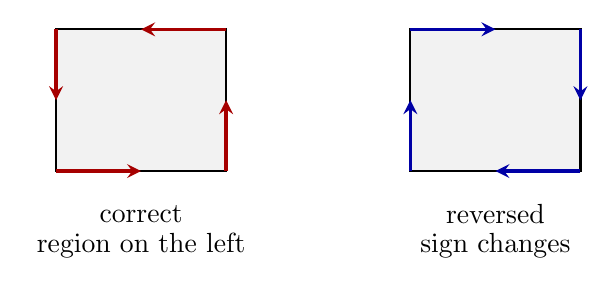
\begin{tikzpicture}[scale=0.9, >=stealth]
    \begin{scope}
        \draw[fill=gray!10, thick] (0,0) rectangle (2.4,2.0);
        \draw[->, very thick, red!65!black] (0,0) -- (1.2,0);
        \draw[->, very thick, red!65!black] (2.4,0) -- (2.4,1.0);
        \draw[->, very thick, red!65!black] (2.4,2.0) -- (1.2,2.0);
        \draw[->, very thick, red!65!black] (0,2.0) -- (0,1.0);
        \node at (1.2,-0.6) {correct};
        \node at (1.2,-1.05) {region on the left};
    \end{scope}

    \begin{scope}[shift={(5.0,0)}]
        \draw[fill=gray!10, thick] (0,0) rectangle (2.4,2.0);
        \draw[->, very thick, blue!65!black] (0,0) -- (0,1.0);
        \draw[->, very thick, blue!65!black] (0,2.0) -- (1.2,2.0);
        \draw[->, very thick, blue!65!black] (2.4,2.0) -- (2.4,1.0);
        \draw[->, very thick, blue!65!black] (2.4,0) -- (1.2,0);
        \node at (1.2,-0.6) {reversed};
        \node at (1.2,-1.05) {sign changes};
    \end{scope}
\end{tikzpicture}
\caption{Reversing the boundary direction reverses the boundary integral.}
\end{figure}

\subsection{Missing boundary components around holes}

A hole is not empty bookkeeping.  It creates an inner boundary.

Let
\[
    A=\{(x,y):1\le x^2+y^2\le4\}
\]
be the annulus between the circles of radius \(1\) and \(2\).  Use the standard
orientation
\[
    dx\wedge dy.
\]
The outer boundary is counterclockwise, and the inner boundary is clockwise.

Take the area-measuring form
\[
    \omega=\frac12(-y\,dx+x\,dy).
\]
Then
\[
    d\omega=dx\wedge dy.
\]
So
\[
    \int_A d\omega
    =
    \operatorname{Area}(A)
    =
    4\pi-\pi
    =
    3\pi.
\]

Now compute the boundary integral.  On a counterclockwise circle of radius \(r\),
\[
    x=r\cos t,
    \qquad
    y=r\sin t,
    \qquad
    0\le t\le2\pi.
\]
Then
\[
    dx=-r\sin t\,dt,
    \qquad
    dy=r\cos t\,dt.
\]
Substitute:
\[
\begin{aligned}
    \omega
    &=
    \frac12\left(
    -r\sin t(-r\sin t\,dt)
    +
    r\cos t(r\cos t\,dt)
    \right)\\
    &=
    \frac12r^2\,dt.
\end{aligned}
\]
So a counterclockwise circle of radius \(r\) contributes
\[
    \pi r^2.
\]

The outer circle contributes
\[
    4\pi.
\]
The inner circle has radius \(1\), but it is oriented clockwise, so it contributes
\[
    -\pi.
\]
Therefore
\[
\boxed{
    \int_{\partial A}\omega=4\pi-\pi=3\pi.
}
\]
This matches
\[
    \int_A d\omega=3\pi.
\]

If we forgot the inner boundary, we would get
\[
    4\pi,
\]
which is wrong.

\[
\boxed{
    \text{The boundary of a region with holes has all its boundary components.}
}
\]

The same warning holds in three dimensions.  A solid shell
\[
    b\le x^2+y^2+z^2\le a^2
\]
has two boundary spheres.  The outer sphere is oriented outward from the shell, away
from the origin.  The inner sphere is also oriented outward from the shell, which points
toward the origin.  That sign is exactly what makes flux contributions cancel when the
field has no source inside the shell.

\subsection{Singularities inside the region}

Some forms look harmless on the boundary but fail inside.  Stokes' theorem needs the
form to be defined on an open set containing the whole object \(M\), not only on
\(\partial M\).

Consider the \(1\)-form
\[
    \alpha=
    \frac{-y}{x^2+y^2}\,dx+
    \frac{x}{x^2+y^2}\,dy.
\]
It is defined on
\[
    \mathbb R^2\setminus\{(0,0)\}.
\]
Where it is defined,
\[
    d\alpha=0.
\]

On the unit circle
\[
    C:\quad x=\cos t,\qquad y=\sin t,
    \qquad 0\le t\le2\pi,
\]
we have
\[
    dx=-\sin t\,dt,
    \qquad
    dy=\cos t\,dt.
\]
So
\[
\begin{aligned}
    \alpha
    &=
    (-\sin t)(-\sin t\,dt)+(\cos t)(\cos t\,dt)\\
    &=
    dt.
\end{aligned}
\]
Therefore
\[
\boxed{
    \int_C\alpha=2\pi.
}
\]

A careless argument would say:
\[
    d\alpha=0,
    \qquad
    \text{so }
    \int_C\alpha=0.
\]
But that argument tries to use Stokes' theorem on the unit disk.  The form \(\alpha\)
is not defined at the origin, and the origin lies inside the disk.  The theorem is not
available.

If we remove a small disk around the origin, the theorem works again.  The region is
an annulus:
\[
    \varepsilon\le x^2+y^2\le1.
\]
On that annulus,
\[
    d\alpha=0.
\]
The outer boundary contributes
\[
    2\pi.
\]
The inner boundary is clockwise, so it contributes
\[
    -2\pi.
\]
The total boundary integral is
\[
    2\pi-2\pi=0,
\]
matching
\[
    \int_{\text{annulus}}d\alpha=0.
\]

The singularity did not disappear.  We turned it into a boundary component.

\[
\boxed{
    \text{A missing point inside can be detected by a loop around it.}
}
\]

There is a three-dimensional version of the same warning.  Let
\[
    r=\sqrt{x^2+y^2+z^2}
\]
and consider the flux \(2\)-form
\[
    \Psi=
    \frac{x}{r^3}\,dy\wedge dz
    +
    \frac{y}{r^3}\,dz\wedge dx
    +
    \frac{z}{r^3}\,dx\wedge dy.
\]
This is the flux form of
\[
    \mathbf G=\frac{(x,y,z)}{r^3}.
\]
The field is not defined at the origin.  Away from the origin,
\[
    d\Psi=0.
\]

Yet the outward flux through a sphere of radius \(a\) is
\[
    4\pi.
\]
It would be wrong to apply the divergence theorem to the whole ball and conclude
zero flux.  The form is not defined at the origin.  If we remove a smaller ball around
the origin, the outer flux \(4\pi\) and inner flux \(-4\pi\) cancel, just as they should.

A singularity inside a region behaves like a source the ordinary derivative does not see,
because the ordinary derivative is not defined there.

\subsection{Smoothness assumptions and piecewise smooth objects}

The theorem also asks for the form to be smooth enough.  In this book, the safe
condition is:
\[
    \omega\text{ has }C^1\text{ coefficients}
\]
on an open set containing \(M\).

A jump can hide an internal boundary.

Let
\[
    R=[-1,1]\times[-1,1],
\]
and define
\[
    H(y)=
    \begin{cases}
    0, & y<0,\\
    1, & y\ge 0.
    \end{cases}
\]
Consider the \(1\)-form
\[
    \omega=H(y)\,dx.
\]
This form is not continuous across the line
\[
    y=0.
\]
It is certainly not \(C^1\).

If we ignore the jump and look only on the two open halves of the square, then \(H\)
is constant on each half, so a careless computation would say
\[
    d\omega=0.
\]
That would suggest
\[
    \int_{\partial R}\omega=0.
\]

But compute the boundary integral directly.  On the bottom edge, \(y=-1\), so
\[
    H(y)=0,
\]
and the contribution is \(0\).  On the right and left edges,
\[
    dx=0,
\]
so the contribution is \(0\).  On the top edge, \(y=1\), and the positive boundary
orientation travels from
\[
    x=1
    \quad\text{to}\quad
    x=-1.
\]
There
\[
    H(y)=1,
\]
so the top contributes
\[
    \int_1^{-1}dx=-2.
\]
Thus
\[
\boxed{
    \int_{\partial R}\omega=-2.
}
\]

The jump along \(y=0\) is hiding an internal edge.  The \(C^1\) theorem is not designed
to ignore that edge.  More advanced versions of Stokes' theorem can handle jumps, but
then the jump contributes its own term.

Smoothness of the boundary is a separate issue.

A rectangle is allowed even though it has corners.  Its boundary is made of finitely
many smooth edges.  A box is allowed even though it has edges and corners.  Its
boundary is made of finitely many smooth faces.  That is what piecewise smooth
means.

Corners do not create extra terms.  Interior shared edges cancel.

For example, split the rectangle
\[
    [0,2]\times[0,1]
\]
into two rectangles:
\[
    R_1=[0,1]\times[0,1],
    \qquad
    R_2=[1,2]\times[0,1].
\]
The shared edge is
\[
    x=1,\qquad 0\le y\le1.
\]
As part of \(\partial R_1\), that edge is traveled upward.  As part of \(\partial R_2\),
the same edge is traveled downward.  The two line integrals cancel for every
\(1\)-form:
\[
    \int_{\text{shared edge from }R_1}\omega
    +
    \int_{\text{shared edge from }R_2}\omega
    =
    0.
\]
Only the outside boundary survives.

So the warning is not ``corners are bad.''  The warning is more precise:

\[
\boxed{
\begin{array}{c}
\text{finite piecewise smooth geometry is allowed,}\\[1mm]
\text{but jumps, singularities, and wild boundaries are not covered by the basic theorem.}
\end{array}
}
\]

\subsection{The checklist}

Before using
\[
    \int_{\partial M}\omega=\int_M d\omega,
\]
check the grammar.

\[
\begin{array}{c|l}
\text{Check} & \text{Question} \\ \hline
\text{Degree} &
\omega\text{ has degree }\dim M-1\text{?}\\[1mm]
\text{Boundary} &
\text{Is every boundary component included?}\\[1mm]
\text{Orientation} &
\text{Does }\partial M\text{ have the induced orientation?}\\[1mm]
\text{Domain} &
\omega\text{ is defined on an open set containing }M\text{?}\\[1mm]
\text{Smoothness} &
\omega\text{ has }C^1\text{ coefficients where needed?}\\[1mm]
\text{Geometry} &
M\text{ and }\partial M\text{ are compact and piecewise smooth?}
\end{array}
\]

When one of these checks fails, the formula may still have a more advanced version.
But the missing condition must be paid for.  A reversed orientation pays with a minus
sign.  A missing hole pays with an extra boundary component.  A singularity pays by
acting like a hidden source.  A jump pays by creating an internal edge or sheet.

This is why the generalized Stokes theorem is both simple and strict.  It gives one
sentence for the Fundamental Theorem of Calculus, Green's theorem, Stokes' theorem,
and the divergence theorem.  But the sentence only works when every word is read
correctly.

The chapter review will turn this into practice: translate the old vector formulas into
forms, choose the right boundary, and decide which side of the theorem is easier to
compute.  After that, the same boundary idea begins to move in time.  A conserved
quantity changes inside a region only because it flows through the boundary.  That is
where Stokes' theorem becomes the language of conservation laws.


\subsection{Boundary orientation reversed}
% TODO

\subsection{Missing boundary components around holes}
% TODO

\subsection{Singularities inside the region}
% TODO

\subsection{Smoothness assumptions and piecewise smooth objects}
% TODO

\section{Chapter review and capstone problems}
\label{sec:18.10}

Section \ref{sec:18.9} was a warning label.  It showed that Stokes' theorem is simple,
but not loose.  The boundary must have the right orientation.  Holes must be counted.
Singularities cannot be ignored.  The form must be smooth enough for \(d\omega\) to
mean what we say it means.

Now we put the chapter in working order.

The whole chapter can be read as one sentence:
\[
\boxed{
    \int_{\partial M}\omega=\int_M d\omega.
}
\]
The rest is translation.

\subsection{The one sentence, read slowly}

The symbol \(M\) is the object with an inside.  It may be an interval, a plane region,
a surface, or a solid.

The symbol \(\partial M\) is its oriented boundary.

The form \(\omega\) lives on the boundary.  The form \(d\omega\) lives inside.

\[
\begin{array}{c|c|c|c}
\dim M & M & \partial M & \omega \\ \hline
1 & \text{interval} & \text{signed endpoints} & 0\text{-form}\\[1mm]
2 & \text{plane region} & \text{oriented boundary curve} & 1\text{-form}\\[1mm]
2 & \text{surface in space} & \text{oriented boundary curve} & 1\text{-form}\\[1mm]
3 & \text{solid region} & \text{outward-oriented boundary surface} & 2\text{-form}
\end{array}
\]

The degree of \(\omega\) is always one less than the dimension of \(M\):
\[
    \deg \omega=\dim M-1.
\]
Then \(d\omega\) has degree
\[
    \deg(d\omega)=\dim M,
\]
so it can be integrated over \(M\).

That is why the dimensions match.

\subsection{A final worked translation}

Let \(C\) be the unit circle in the plane \(z=0\), oriented counterclockwise when viewed
from above:
\[
    C:\quad x^2+y^2=1,\qquad z=0.
\]
Take the \(1\)-form
\[
    \omega=-y\,dx+x\,dy+z\,dz.
\]

First compute the boundary integral directly.  Parametrize \(C\) by
\[
    x=\cos t,\qquad y=\sin t,\qquad z=0,
    \qquad 0\le t\le 2\pi.
\]
Then
\[
    dx=-\sin t\,dt,
    \qquad
    dy=\cos t\,dt,
    \qquad
    dz=0.
\]
So
\[
\begin{aligned}
    \omega
    &=
    -\sin t(-\sin t\,dt)+\cos t(\cos t\,dt)+0\\
    &=
    (\sin^2 t+\cos^2 t)\,dt\\
    &=
    dt.
\end{aligned}
\]
Therefore
\[
\boxed{
    \int_C\omega=2\pi.
}
\]

Now compute using Stokes' theorem.  The exterior derivative is
\[
\begin{aligned}
    d\omega
    &=
    d(-y\,dx)+d(x\,dy)+d(z\,dz)\\
    &=
    -dy\wedge dx+dx\wedge dy+0\\
    &=
    2\,dx\wedge dy.
\end{aligned}
\]

Let \(D\) be the flat unit disk in the plane \(z=0\), oriented upward.  Its boundary is
\(C\).  Then
\[
\begin{aligned}
    \int_C\omega
    &=
    \int_D d\omega\\
    &=
    \int_D 2\,dx\wedge dy\\
    &=
    2\operatorname{Area}(D)\\
    &=
    2\pi.
\end{aligned}
\]

But the flat disk was not special.  Let \(S\) be the downward-opening paraboloid cap
\[
    z=1-x^2-y^2,
    \qquad
    x^2+y^2\le1,
\]
oriented upward.  Its boundary is the same circle \(C\), with the same induced
orientation.  Stokes' theorem gives
\[
    \int_C\omega=\int_S d\omega.
\]
Since
\[
    d\omega=2\,dx\wedge dy,
\]
the surface integral measures twice the signed area of the shadow of \(S\) on the
\(xy\)-plane.  With upward orientation, that shadow is the unit disk with positive
orientation.  Hence
\[
\boxed{
    \int_S d\omega=2\pi.
}
\]

The flat disk and the curved cap give the same answer because the boundary is the
same.  Stokes' theorem says the integral of \(d\omega\) over a surface depends only on
the boundary, as long as \(\omega\) is defined on the region swept between the surfaces.

\subsection{The formulas to keep}

The formulas below are not separate miracles.  They are the same theorem in different
degrees.

\[
\boxed{
    df=f_x\,dx+f_y\,dy+f_z\,dz.
}
\]

For a plane \(1\)-form,
\[
    \omega=P\,dx+Q\,dy,
\]
\[
\boxed{
    d\omega=(Q_x-P_y)\,dx\wedge dy.
}
\]

For a space \(1\)-form,
\[
    \omega=P\,dx+Q\,dy+R\,dz,
\]
\[
\boxed{
\begin{aligned}
    d\omega
    &=
    (R_y-Q_z)\,dy\wedge dz\\
    &\quad+
    (P_z-R_x)\,dz\wedge dx\\
    &\quad+
    (Q_x-P_y)\,dx\wedge dy.
\end{aligned}
}
\]
This is the flux \(2\)-form of
\[
    \nabla\times(P,Q,R).
\]

For a flux \(2\)-form,
\[
    \Phi=P\,dy\wedge dz+Q\,dz\wedge dx+R\,dx\wedge dy,
\]
\[
\boxed{
    d\Phi=(P_x+Q_y+R_z)\,dx\wedge dy\wedge dz.
}
\]
This is the divergence volume form.

The orientation rules are just as important:

\[
\begin{array}{c|c}
\text{Object} & \text{Induced boundary orientation} \\ \hline
[a,b] & \partial[a,b]=\{b\}-\{a\}\\[1mm]
\text{plane region} & \text{walk so the region stays on the left}\\[1mm]
\text{oriented surface} & \text{right-hand rule}\\[1mm]
\text{solid region} & \text{outward-oriented boundary surface}
\end{array}
\]

\subsection{Concept check}

\begin{enumerate}
\item What degree should \(\omega\) have if \(M\) is a surface?

\item What degree should \(\omega\) have if \(M\) is a solid?

\item Why is the boundary of an interval written
\[
    \{b\}-\{a\}
\]
instead of just
\[
    \{a,b\}?
\]

\item For a positively oriented plane region, why is an inner boundary around a hole
walked clockwise?

\item If a surface is oriented upward, how do you determine the positive direction of
its boundary curve?

\item What does
\[
    \partial(\partial M)=\emptyset
\]
mean for a solid box?

\item What does
\[
    d^2=0
\]
say in vector language for
\[
    d(df)?
\]

\item What does
\[
    d^2=0
\]
say in vector language for
\[
    d(d(P\,dx+Q\,dy+R\,dz))?
\]

\item Why can a form with \(d\omega=0\) still have a nonzero integral around a closed
curve?

\item Why must Stokes' theorem require \(\omega\) to be defined on the inside region,
not only on the boundary?
\end{enumerate}

\subsection{Skills: translating between vector calculus and forms}

\begin{enumerate}
\item Compute \(df\) for
\[
    f(x,y,z)=x^2y+yz^3-\cos x.
\]

\item Compute \(d\omega\) for the plane \(1\)-form
\[
    \omega=(x^2-y)\,dx+(xy+3y^2)\,dy.
\]

\item Compute \(d\omega\) for the space \(1\)-form
\[
    \omega=yz\,dx+xz\,dy+xy\,dz.
\]
Identify the vector field whose flux form is \(d\omega\).

\item Compute \(d\Phi\) for
\[
    \Phi=x^2\,dy\wedge dz+y^2\,dz\wedge dx+z^2\,dx\wedge dy.
\]
Translate your answer into divergence language.

\item Let
\[
    \mathbf F=(P,Q,R).
\]
Write the work \(1\)-form of \(\mathbf F\).  Then write \(d\omega_{\mathbf F}\) and
identify the vector field it represents.

\item Let
\[
    \mathbf F=(P,Q,R).
\]
Write the flux \(2\)-form of \(\mathbf F\).  Then write \(d\Phi_{\mathbf F}\) and identify
its coefficient.

\item Let \(R\) be a positively oriented plane region.  Translate
\[
    \oint_{\partial R}\mathbf F\cdot d\mathbf r
\]
into a \(1\)-form integral.

\item Let \(E\) be a solid region.  Translate
\[
    \iint_{\partial E}\mathbf F\cdot\widehat{\mathbf n}_{\mathrm{out}}\,dS
\]
into a \(2\)-form integral.
\end{enumerate}

\subsection{Practice problems}

\begin{enumerate}
\item Let
\[
    I=[-2,5]
\]
with the usual orientation, and let
\[
    f(x)=x^3-4x.
\]
Compute both sides of
\[
    \int_{\partial I}f=\int_I df.
\]

\item Let
\[
    R=[0,3]\times[0,2]
\]
with positive orientation, and let
\[
    \omega=(y^2+x)\,dx+x^2\,dy.
\]
Compute
\[
    \int_{\partial R}\omega
\]
using Green's theorem.

\item Compute the same integral in Problem \(2\) directly by integrating along the four
sides of the rectangle.

\item Let \(C\) be the positively oriented boundary of the triangle with vertices
\[
    (0,0),\qquad (4,0),\qquad (0,3).
\]
Compute
\[
    \int_C x\,dy.
\]
Explain why this integral gives the area of the triangle.

\item Let
\[
    A=\{(x,y):1\le x^2+y^2\le9\}
\]
with the standard orientation.  Compute
\[
    \int_{\partial A}x\,dy.
\]
Be careful with the orientation of the inner boundary.

\item Let
\[
    \omega=-\frac y2\,dx+\frac x2\,dy.
\]
Use Green's theorem to compute
\[
    \int_{\partial R}\omega
\]
when \(R\) is the ellipse
\[
    \frac{x^2}{9}+\frac{y^2}{4}\le1.
\]

\item Let \(S\) be the upper hemisphere
\[
    x^2+y^2+z^2=4,
    \qquad z\ge0,
\]
oriented upward.  Its boundary is the circle
\[
    x^2+y^2=4,\qquad z=0.
\]
Use Stokes' theorem to compute
\[
    \int_{\partial S}(-y\,dx+x\,dy).
\]

\item Let \(S\) be any smooth upward-oriented surface whose boundary is the circle
\[
    x^2+y^2=1,\qquad z=0.
\]
Use Stokes' theorem to compute
\[
    \int_S 3\,dx\wedge dy.
\]

\item Let \(E\) be the box
\[
    [0,1]\times[0,2]\times[0,3],
\]
and let
\[
    \Phi=x\,dy\wedge dz+y\,dz\wedge dx+z\,dx\wedge dy.
\]
Compute
\[
    \int_{\partial E}\Phi
\]
using the divergence theorem.

\item Compute the same integral in Problem \(9\) by adding the six face integrals.

\item Let \(B_a\) be the ball of radius \(a\) centered at the origin.  Use the divergence
theorem to compute the outward flux of
\[
    \mathbf F=(x,y,z)
\]
through
\[
    \partial B_a.
\]

\item Let
\[
    \mathbf F=(y,z,x).
\]
Compute the outward flux of \(\nabla\times\mathbf F\) through any closed surface
\(\partial E\), assuming \(\mathbf F\) is defined on a region containing \(E\).

\item Let
\[
    \alpha=
    \frac{-y}{x^2+y^2}\,dx+
    \frac{x}{x^2+y^2}\,dy.
\]
Compute
\[
    \int_C\alpha
\]
where \(C\) is the unit circle oriented counterclockwise.  Explain why this does not
contradict Green's theorem.

\item Let
\[
    \mathbf G=\frac{(x,y,z)}{(x^2+y^2+z^2)^{3/2}}.
\]
Compute its outward flux through the sphere
\[
    x^2+y^2+z^2=a^2.
\]
Explain why the divergence theorem cannot be applied to the whole ball.

\item Let
\[
    \omega=x\,dy
\]
on the square
\[
    R=[0,1]\times[0,1].
\]
Compute
\[
    \int_{\partial R}\omega
\]
with positive orientation, and then compute the integral with the clockwise orientation.
What changed?

\item Let \(S\) be the flat disk
\[
    x^2+y^2\le1,\qquad z=0,
\]
oriented downward.  What is the induced orientation on \(\partial S\)?  Compute
\[
    \int_{\partial S}(-y\,dx+x\,dy).
\]

\item Let \(E\) be the spherical shell
\[
    1\le x^2+y^2+z^2\le4.
\]
Describe the induced orientations on the two boundary spheres.

\item Let
\[
    \Psi=
    \frac{x}{r^3}\,dy\wedge dz+
    \frac{y}{r^3}\,dz\wedge dx+
    \frac{z}{r^3}\,dx\wedge dy,
    \qquad
    r=\sqrt{x^2+y^2+z^2}.
\]
Use the shell in Problem \(17\) to explain why
\[
    \int_{\partial E}\Psi=0,
\]
even though each boundary sphere has nonzero flux.

\item Suppose
\[
    \omega=d\eta
\]
on a region containing a compact oriented surface \(S\) with no boundary.  Prove that
\[
    \int_S\omega=0.
\]

\item Suppose
\[
    \Phi=d\omega
\]
on a region containing a solid \(E\).  Prove that
\[
    \int_{\partial E}\Phi=0.
\]
Translate this into a vector calculus statement.
\end{enumerate}

\subsection{Capstone project: derive the four classical theorems from one statement}

The goal of this project is to start with
\[
    \int_{\partial M}\omega=\int_M d\omega
\]
and recover the four classical theorems.

For each row below, fill in the missing details.

\[
\begin{array}{c|c|c|c}
\text{Name} & M & \omega & d\omega \\ \hline
\text{Fundamental Theorem of Calculus}
& [a,b]
& f
& df
\\[1mm]
\text{Green's theorem}
& R\subset\mathbb R^2
& P\,dx+Q\,dy
& (Q_x-P_y)\,dx\wedge dy
\\[1mm]
\text{Classical Stokes' theorem}
& S\subset\mathbb R^3
& P\,dx+Q\,dy+R\,dz
& \Phi_{\nabla\times\mathbf F}
\\[1mm]
\text{Divergence theorem}
& E\subset\mathbb R^3
& \Phi_{\mathbf F}
& (\nabla\cdot\mathbf F)\,dx\wedge dy\wedge dz
\end{array}
\]

Write one page for each theorem.  Each page should include:

\begin{enumerate}
\item the object \(M\),
\item its oriented boundary \(\partial M\),
\item the form \(\omega\),
\item the exterior derivative \(d\omega\),
\item the forms version of the theorem,
\item the classical vector-calculus version, if there is one,
\item one warning about orientation, holes, or singularities.
\end{enumerate}

The project is not about memorizing four formulas.  It is about showing that the four
formulas are the same sentence with different nouns.

\subsection{Capstone project: one boundary, three surfaces}

Let \(C\) be the unit circle
\[
    x^2+y^2=1,\qquad z=0,
\]
oriented counterclockwise when viewed from above.  Let
\[
    \omega=-y\,dx+x\,dy.
\]

Compute
\[
    \int_C\omega
\]
in four ways.

\begin{enumerate}
\item Directly parametrize \(C\).

\item Use the flat disk
\[
    D:\quad x^2+y^2\le1,\qquad z=0,
\]
oriented upward.

\item Use the upper hemisphere
\[
    S_1:\quad x^2+y^2+z^2=1,\qquad z\ge0,
\]
oriented outward.

\item Use the cone
\[
    S_2:\quad z=1-\sqrt{x^2+y^2},\qquad x^2+y^2\le1,
\]
oriented upward.
\end{enumerate}

In your write-up, explain why the three surface computations agree.  Then reverse the
orientation of \(C\) and describe what changes.

\subsection{Capstone project: find the hidden mistake}

Each statement below is wrong or incomplete.  Find the missing condition or sign error.

\begin{enumerate}
\item Since
\[
    d\left(
    \frac{-y}{x^2+y^2}\,dx+
    \frac{x}{x^2+y^2}\,dy
    \right)=0,
\]
the integral of this form around the unit circle must be \(0\).

\item The boundary of an annulus is only its outer circle.

\item If a disk is oriented upward, we may choose either clockwise or counterclockwise
orientation on its boundary and Stokes' theorem will still hold.

\item Since the disk
\[
    x^2+y^2\le1,\qquad z=0
\]
has no volume, the divergence theorem says the flux of \((0,0,1)\) through it is \(0\).

\item Since
\[
    \nabla\cdot\left(\frac{(x,y,z)}{r^3}\right)=0
\]
away from the origin, the outward flux through a sphere around the origin is \(0\).

\item A cube surface has edges, so as a surface it must have a boundary curve.

\item If
\[
    \nabla\times\mathbf F=\mathbf 0,
\]
then every line integral of \(\mathbf F\cdot d\mathbf r\) around a closed curve is \(0\),
even if the domain has holes.

\item If two surfaces have the same boundary, then
\[
    \int_S \Phi
\]
must be the same for every \(2\)-form \(\Phi\).
\end{enumerate}

\subsection{Where the theorem leads next}

Stokes' theorem compares what happens on a boundary with what happens inside:
\[
    \int_{\partial M}\omega=\int_M d\omega.
\]
That sentence is already a conservation law in disguise.

Imagine a pollutant spread through a fixed tank \(E\).  Let
\[
    \rho(x,y,z,t)
\]
be its density at time \(t\).  The amount inside the tank is
\[
    \int_E \rho\,dx\wedge dy\wedge dz.
\]
If pollutant flows out through the boundary, the amount inside decreases.  Let
\[
    \Phi_{\mathbf J}
    =
    J_1\,dy\wedge dz+J_2\,dz\wedge dx+J_3\,dx\wedge dy
\]
be the outward flux \(2\)-form of the flux vector field
\[
    \mathbf J=(J_1,J_2,J_3).
\]
Then the boundary loss is
\[
    \int_{\partial E}\Phi_{\mathbf J}.
\]
Stokes' theorem turns that boundary flux into an interior integral:
\[
    \int_{\partial E}\Phi_{\mathbf J}
    =
    \int_E d\Phi_{\mathbf J}
    =
    \int_E (\nabla\cdot\mathbf J)\,dx\wedge dy\wedge dz.
\]

So the balance law becomes
\[
\boxed{
    \frac{d}{dt}
    \int_E \rho\,dx\wedge dy\wedge dz
    =
    -
    \int_{\partial E}\Phi_{\mathbf J}.
}
\]
Using Stokes' theorem,
\[
\boxed{
    \frac{d}{dt}
    \int_E \rho\,dx\wedge dy\wedge dz
    =
    -
    \int_E d\Phi_{\mathbf J}.
}
\]

\begin{figure}[h]
\centering
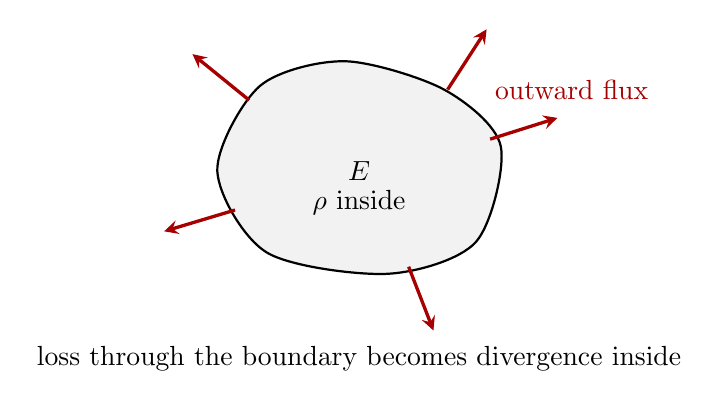
\begin{tikzpicture}[scale=0.9, >=stealth]
    \draw[fill=gray!10, thick]
        plot[smooth cycle] coordinates {
            (-2.0,0.0)
            (-1.4,1.2)
            (-0.2,1.55)
            (1.2,1.15)
            (2.0,0.35)
            (1.65,-1.0)
            (0.4,-1.45)
            (-1.3,-1.15)
        };

    \node at (0,0) {\(E\)};
    \node at (0,-0.45) {\(\rho\) inside};

    \draw[->, very thick, red!65!black] (1.85,0.45) -- (2.8,0.75);
    \draw[->, very thick, red!65!black] (1.25,1.15) -- (1.8,2.0);
    \draw[->, very thick, red!65!black] (-1.55,1.0) -- (-2.35,1.65);
    \draw[->, very thick, red!65!black] (-1.75,-0.55) -- (-2.75,-0.85);
    \draw[->, very thick, red!65!black] (0.7,-1.35) -- (1.05,-2.25);

    \node[red!65!black] at (3.0,1.15) {outward flux};
    \node at (0,-2.65) {loss through the boundary becomes divergence inside};
\end{tikzpicture}
\caption{A conservation law compares change inside a region with flux through its boundary.}
\end{figure}

If this balance holds for every small region \(E\), then the integrands must balance
locally:
\[
\boxed{
    \rho_t+\nabla\cdot\mathbf J=0.
}
\]
This is the continuity equation.

The next chapter follows that idea.  Stokes' theorem was a theorem about space:
boundary versus interior.  Conservation laws add time.  A quantity changes inside a
region only because it is created, destroyed, or carried through the boundary.  The
same boundary principle that unified calculus now becomes the language of fluids,
heat, waves, and fields.